\documentclass[nofootinbib,reprint,english]{revtex4-1}

% language
\usepackage[utf8]{inputenc}
\usepackage[english]{babel}

% standard setup
\usepackage{physics,amssymb,array}
\usepackage{xcolor,graphicx,hyperref}
\usepackage{tikz,listings,multirow}
\usepackage{algpseudocode,algorithm}
\usepackage{subcaption}
\usepackage{enumitem}

% tikz libraries
\usetikzlibrary{matrix}

% hyperref coloring
\hypersetup{ %
  colorlinks,
  linkcolor={red!50!black},
  citecolor={blue!50!black},
  urlcolor={blue!80!black}}

% lstlisting coloring
\lstset{ %
  inputpath=,
  backgroundcolor=\color{white!88!black},
  basicstyle={\ttfamily\scriptsize},
  commentstyle=\color{magenta},
  language=Python,
  tabsize=2,
  numbers=left,
  stringstyle=\color{green!55!black},
  frame=single,
  keywordstyle=\color{blue},
  showstringspaces=false,
  columns=fullflexible,
  keepspaces=true}

\DeclareTextSymbolDefault{\dh}{T1}

% no "do"'s or "then"'s
\algdef{SE}[FOR]{NoDoFor}{EndFor}[1]{\algorithmicfor\ #1}{\algorithmicend\ \algorithmicfor}
\algdef{SE}[FORALL]{NoDoForAll}{EndFor}[1]{\algorithmicfor\ #1}{\algorithmicend\ \algorithmicfor}
\algdef{SE}[IF]{NoThenIf}{EndIf}[1]{\algorithmicif\ #1}{\algorithmicend\ \algorithmicif}

% spin-configuration table columns
\newcolumntype{M}[1]{>{\centering\arraybackslash}m{#1}}
\newcolumntype{N}{@{}m{0pt}@{}}

% shortcuts
\newcommand{\hatHH}{\hat{\mathcal{H}}}
\newcommand{\HH}{\mathcal{H}}
\newcommand{\Sspace}{\mathcal{S}}

\begin{document}
% titlepage
\title{FYS3150 Computational Physics - Project 5\\Variational Monte Carlo}
\author{Nils Johannes Mikkelsen}
\date{\today}
\noaffiliation
\begin{abstract}

\end{abstract}
\maketitle
All material written for project 5 may be found at:\\
{\scriptsize\url{https://github.com/njmikkelsen/comphys2018/tree/master/Project5}}
\section{Introduction}

\section{Theory}
\subsection{Quantum Mechanics - Miscellaneous}
The reader is assumed to be familiar with most of the basic features of quantum mechanics such as Dirac notation, the notion of kets and Hilbert spaces, quantum spin, composite systems, etc. Nonetheless, the following sections introduce some of the basic aspects of quantum mechanics that are readily applied and studied in this project.
\subsubsection{Notation}
First and foremost, kets and bras are depicted as usual, e.g. \(\ket{\psi}\) and \(\bra{\phi}\). The hermiation conjugate of some object \(c\) is denoted by a dagger: \(c^\dagger\). In general, operators are denoted by upper case letters and constants by lower case letters, although exceptions such as the canonical operators and ladder operators do exist. Furthermore, operators are denoted by an additional ''hat" in the absence of a particular basis. For example, the canonical operators \(\hat{\vb{r}}\) and \(\hat{\vb{p}}\) expressed in the position basis \(\ket{\vb{r}}\), are given by:
\begin{equation}
\vb{r}\qand\vb{p}=-i\hbar\nabla
\end{equation}
Moreover, the single-system Hamiltonian for a system with mass \(m\) in a potential \(V\):
\begin{subequations}
\begin{align}
\hatHH=\frac{\hat{\vb{p}}^2}{2m}+V(\hat{\vb{r}},\hat{\vb{p}})\\
\intertext{thus takes the following form in the position basis:}
\HH=\frac{-\hbar^2}{2m}\nabla^2+V(\vb{r},-i\hbar\nabla)
\end{align}
\end{subequations}
Unless otherwise specified, all operators are expressed in the continuous position basis. Provided a classical operator \(O\), the corresponding quantum operator \(\hat{O}\) is found by inserting the canonical operators: \(\hat{O}=O(\hat{\vb{r}},\hat{\vb{p}})\).

Composite systems are denoted either as a tensor product, say \(\ket{\psi}\otimes\ket{\phi}\) , or using some form of compact notation \(\ket{\psi,\phi}\), depending on the system in question. This report will favour a compact notation in cases where such notation is natural. Each component of a composite system is considered a degree of freedom, be it different spatial degrees of freedom of the same system or completely unrelated degrees of freedom (e.g. an electron's position and spin). The Hamiltonian of a composite system with \(N\) degrees of freedom is equal to the sum of the individual Hamiltonians for each component plus the interaction:
\begin{equation}\label{eq:Composite_Hamiltonian}
\hatHH_\text{composite}=\sum_{i=1}^N\hatHH_{i}+\hatHH_\text{interaction}
\end{equation}
where \(\hatHH_\text{interaction}\) encompases all interactions between the \(N\) degrees of freedom.

For infinite-dimensional Hilbert spaces, the inner product between \(\ket{\psi}\) and \(\ket{\phi}\) is
\begin{equation}
\braket{\psi}{\phi}=\int\dd[3]{\vb{r}}\psi(\vb{r})^*\phi(\vb{r})
\end{equation}
Similarly, the expected value of some operator \(\hat{A}\) for a system in a state \(\ket{\psi}\) is
\begin{equation}\label{eq:expected_value_of_operator}
\bra{\psi}\hat{A}\ket{\psi}=\int\dd[3]{\vb{r}}\psi(\vb{r})^*\hat{A}\psi(\vb{r})
\end{equation}
In case \(\ket{\psi}\) is an eigenket of \(\hat{A}\) with corresponding eigenvalue \(a\), \eqref{eq:expected_value_of_operator} is simplified to
\begin{equation}\label{eq:expected_value_of_operator_eigenstate}
\bra{\psi}\hat{A}\ket{\psi}=\bra{\psi}a\ket{\psi}=a\braket{\psi}{\psi}=a
\end{equation}
assuming \(\ket{\psi}\) is normalised. Expanding the integral in \eqref{eq:expected_value_of_operator_eigenstate} one finds that the wave functions simplify to \(\abs{\psi(\vb{r})}^2\): the probability density of finding the system at \(\vb{r}\).
\subsubsection{Natural (atomic) units}
To simplify the mathematics and computations in this project, natural atomic units will be adapted. The particular system of units adapted in this project define
\begin{equation}
\hbar=e=m_e=k_e=k_B\qand c=\frac{1}{\alpha}\approx137
\end{equation}
where \(e\) is the elementary charge, \(k_e\) is Coulomb's constant, \(k_B\) is the Boltzmann constant and \(\alpha\) is the fine structure constant. Written in terms of these units the Hamiltonian takes the form
\begin{equation}
\hatHH=-\frac{1}{2m}\nabla^2+V(\vb{r},-i\nabla)
\end{equation}
where \(m\) is given in terms of \(m_e\). Energy is expressed in units of ``Hartree energy'' \(E_h\):
\[\alpha=\frac{k_ee^2}{\hbar c}\implies E_h=\frac{m_e{k_e}^2e^4}{\hbar^2}=m_ec^2\alpha^2=1\]

\subsubsection{The variational principle \& method}
The variational principle (not to be confused with the variational method, see below) is a simple statement that is true for all quantum systems. It states that the expected energy of a quantum system in a state \(\ket{\psi}\) is greater than or equal to the ground state energy:
\begin{equation}\label{eq:variational_principle}
E_g\leq\frac{\bra{\psi}\hatHH\ket{\psi}}{\braket{\psi}}
\end{equation}
Here \(\ket{\psi}\) is not necessarily normalized (which is way the expected energy is divided by the norm). The equation becomes an equality only when \(\ket{\psi}\) is the ground state. 

The variational principle is the basis for the \emph{variational method}, which exploits the simplicity of the varitional principle in order to approximate the ground state energy. The primary problem is to study some Hamiltonian \(\hatHH\) whose energy eigenkets are unknown. The idea is to introduce a so-called \emph{trial state} \(\ket{\psi_T(\gamma)}\), which is dependent on some parameter \(\gamma\) (which is not necessarily scalar). If chosen correctly, the trial state may be able to reproduce the functional shape of the ground state, thus providing an approximate upper bound \(E_T\) of the ground state energy. The variational method is actually an umbrella term for several methods, however, their underlying idea is more or less the same. The process is most easily shown as an algorithm:
\begin{algorithm}[H]
\caption{The Varitational Method}\label{algo:varitational_method}
\begin{algorithmic}[1]
\State Suggest a trial state \(\ket{\psi_T(\gamma)}\).
\State Compute the trial energy \(E_T\) as a function of \(\gamma\):
\[E_T(\gamma)=\frac{\bra{\psi_T(\gamma)}\hatHH\ket{\psi_T(\gamma)}}{\braket{\psi_T(\gamma)}}\]
\State Minimise \(E_T\) with respect to \(\gamma\).
\State Choose the optimal \(\ket{\psi_T(\gamma)}\) based on the \(\gamma\) that minimises \(E_T\).

\noindent The resulting optimal \(E_T\) is an upper bound on the ground state energy, while the corresponding trial state is the optimal approximation of the ground state.
\end{algorithmic}
\end{algorithm}
Due to computational aspects, a common variant of the algorithm is to have the process of minimsation of \(E_T\) be integrated in a loop over different parameters \(\gamma\).
\subsubsection{The Coulomb interaction}
An interesting, although somewhat discouraging, reality is that one of the fundamental interactions of nature, the Coulomb interaction, is more or less analytically unsolvable for everything but the simplest of systems. The Hydrogen is one such system in which the interaction is perfectly solvable. On the other hand, the second simplest element, Helium, is not. The problem arises from the electron-electron interaction:
\begin{equation}\label{eq:electron_electron_Coulomb_interaction}
V_{e^-e^-}=\frac{k_ee^2}{|\vb{r}_1-\vb{r}_2|}=\frac{1}{|\vb{r}_1-\vb{r}_2|}
\end{equation}
where \(\vb{r}_1\) and \(\vb{r}_2\) are the positions of electron 1 and 2.
\subsection{Quantum Mechanics - The Harmonic Oscillator}
The harmonic oscillator is one of the finest achivements of quantum mechanics with applications in many areas of physics and other sciences. The following section will present the algebraic solution to the harmonic oscillator Hamiltonian, and generalise the results to an \(N\)-dimensional system of oscillators.
\subsubsection{The single harmonic oscillator}
The potential energy of a single-degree classical harmonic oscillator with oscillation frequency \(\omega\) is \(V=\frac{1}{2}\omega^2x^2\), it follows that the Hamiltonian for a single-degree quantum harmonic oscillator with mass \(m\) is
\begin{equation}\label{eq:Hamiltonian_harmonic_oscillator}
\hatHH_\text{HO}=\frac{\hat{p}^2}{2m}+\frac{1}{2}\omega^2\hat{x}
\end{equation}
where \(\hat{p}=\hat{\vb{p}}\cdot\vb{e}_x\) is the system's momentum operator. The problem at hand is to find the energy eigenkets of the Hamiltonian. This will be done using the so-called \emph{ladder operators}:\footnote{These operators have several names, e.g. \emph{raising/lowering} operators, \emph{creation/annahilation} operators, etc.}
\begin{subequations}\label{eq:harmonic_oscillator_ladder_operators}
\begin{align}
        \hat{a}&=\frac{1}{\sqrt{2m\omega}}\big(+i\hat{p}+m\omega\hat{x}\big)\\
\hat{a}^\dagger&=\frac{1}{\sqrt{2m\omega}}\big(-i\hat{p}+m\omega\hat{x}\big)
\end{align}
\end{subequations}
One can easily show that the ladder operators satisfy the commutation relation \([\hat{a},\hat{a}^\dagger]=1\). Rewriting \(\hat{x}\) and \(\hat{p}\) in terms of \(\hat{a}\) and \(\hat{a}^\dagger\), one finds that the Hamiltonian can be written as
\begin{equation}
\hatHH_\text{HO}=\omega\bigg(\hat{a}^\dagger\hat{a}+\frac{1}{2}\bigg)=\omega\bigg(\hat{a}\hat{a}^\dagger-\frac{1}{2}\bigg)
\end{equation}
It turns out that the energy eigenkets can be uniquely labelled using a single non-negative integer index \(n\): \(\ket{n}\). Furthermore, the action of ladder operators on the energy eigenkets raises or lowers \(n\) as follows:
\begin{equation}\label{eq:ladder_operations}
\hat{a}\ket{n}=\sqrt{n}\ket{n-1}\qand\hat{a}^\dagger\ket{n}=\sqrt{n+1}\ket{n+1}
\end{equation}
Note that \(n<0\) is avoided as \(\hat{a}\ket{0}=0\).\footnote{This is actually somewhat missleading, but it originates in the derivation of the harmonic oscillator energies. By requiring non-negative energies, one finds that the ``ladder of energy eigenkets'' must be truncated in order to avoid \(\braket{n}<0\). This truncation is also the origin of the index \(n\).} It follows that \(\hat{a}^\dagger\hat{a}\ket{n}=n\ket{n}\) such that
\begin{equation}\label{eq:harmonic_oscillator_energies}
\hatHH_\text{HO}\ket{n}=\omega\bigg(n+\frac{1}{2}\bigg)\ket{n}=E_n\ket{n}
\end{equation}
The energy eigenkets can be uniquely described in terms of \(\ket{0}\) and \(\hat{a}^\dagger\) via
\begin{equation}\label{eq:harmonic_oscillator_eigenkets}
\ket{n}=\frac{\big(\hat{a}^\dagger\big)^n}{\sqrt{n!}}\ket{0}
\end{equation}
where the factorial accounts for the \(\sqrt{n+1}\) scaling in \eqref{eq:ladder_operations}.

\subsubsection{The virial theorem}
The virial theorem is an important result in both classical and quantum mechanics, a simple version of the virial theorem states that the expected total kinetic energy \(\expval{K}\) is proportional to the expected potential energy \(\expval{V}\). Peculiar to the harmonic oscillator, provided an energy eigenstate, the expected total kinetic energy is actually equal to the expected potential energy.

Suppose a quantum system subject to a harmonic potential is in the energy eigenket \(\ket{n}\). The expected kinetic and potential energies are thus
\begin{subequations}
\begin{align}
\expval{K}_n&=\bra{n}\hat{K}\ket{n}=\bra{n}\frac{\hat{p}^2}{2m}\ket{n}\\
\expval{V}_n&=\bra{n}\hat{V}\ket{n}=\bra{n}\frac{1}{2}m\omega^2\hat{x}^2\ket{n}
\end{align}
\end{subequations}
Rewriting \(\hat{x}\) and \(\hat{p}\) in terms of \(\hat{a}\) and \(\hat{a}^\dagger\) results in:
\begin{align*}
\hat{x}^2=\frac{1}{2m\omega}\big(\hat{a}^\dagger+\hat{a}\big)^2\qand\hat{p}^2=-\frac{m\omega}{2}\big(\hat{a}^\dagger-\hat{a}\big)^2
\end{align*}
The ladder operator polynomials are:
\begin{align*}
\big(\hat{a}^\dagger+\hat{a}\big)^2&=\hat{a}^\dagger\hat{a}^\dagger+\hat{a}^\dagger\hat{a}+\hat{a}\hat{a}^\dagger+\hat{a}\hat{a}\\
&=\hat{a}^\dagger\hat{a}^\dagger+\hat{a}\hat{a}+2\hat{a}^\dagger\hat{a}+1\\[0.25cm]
\big(\hat{a}^\dagger-\hat{a}\big)^2&=\hat{a}^\dagger\hat{a}^\dagger-\hat{a}^\dagger\hat{a}-\hat{a}\hat{a}^\dagger+\hat{a}\hat{a}\\
&=\hat{a}^\dagger\hat{a}^\dagger+\hat{a}\hat{a}-2\hat{a}^\dagger\hat{a}-1
\end{align*}
Hence,
\begin{widetext}
\begin{subequations}\label{eq:harmonic_oscillator_kinetic_and_potential_action}
\begin{align}
\hat{K}\ket{n}&=-\frac{\omega}{4}\bigg[\sqrt{(n+1)(n+2)}\ket{n+2}+\sqrt{n(n-1)}\ket{n-2}-2n\ket{n}-\ket{n}\bigg]\\
\hat{V}\ket{n}&=+\frac{\omega}{4}\bigg[\sqrt{(n+1)(n+2)}\ket{n+2}+\sqrt{n(n-1)}\ket{n-2}+2n\ket{n}+\ket{n}\bigg]
\end{align}
\end{subequations}
\end{widetext}
It follows then that
\begin{equation}
\expval{K}_n=\expval{V}_n=\frac{E_n}{2}=\frac{\omega}{2}\bigg(n+\frac{1}{2}\bigg)
\end{equation}
That is, for a single harmonic oscillator with oscillation frequency \(\omega\) in an energy eigenstate, the expected kinetic and potential energy is the same.

In case the harmonic oscillator is not in an energy eigenstate, but in some arbitrary state \(\ket{\psi}\), it is not necessarily the case that \(\expval{K}=\expval{V}\). Consider the fact that the energy eigenkets span the Hilbert space, thereby implying that
\begin{equation}
\ket{\psi}=\sum_n\alpha_n\ket{n}
\end{equation}
for an appropriate choice of \(\alpha_n\). Furthermore, the expected kinetic energy and potential energy is therefore
\begin{subequations}\label{eq:harmonic_oscillator_expected_kinetic_and_potential_generalised}
\begin{align}
\bra{\psi}\hat{K}\ket{\psi}&=\sum_n\sum_m\alpha_n^*\alpha_m\bra{n}\hat{K}\ket{m}\\
\bra{\psi}\hat{V}\ket{\psi}&=\sum_n\sum_m\alpha_n^*\alpha_m\bra{n}\hat{V}\ket{m}
\end{align}
\end{subequations}
It is not immediately obvious from \eqref{eq:harmonic_oscillator_expected_kinetic_and_potential_generalised} whether \(\expval{K}\) is equal to \(\expval{V}\) or not. However if \(\expval{K}=\expval{V}\), then
\begin{align*}
\bra{\psi}\hat{K}\ket{\psi}-\bra{\psi}\hat{V}\ket{\psi}&=\bra{\psi}\big(\hat{K}-\hat{V}\big)\ket{\psi}\\
&=\sum_n\sum_m\alpha_n^*\alpha_m\bra{n}\big(\hat{K}-\hat{V}\big)\ket{m}
\end{align*}
must be equal to zero. The braket can be simplified by inserting \eqref{eq:harmonic_oscillator_kinetic_and_potential_action}:
\[-\frac{\omega}{2}\bigg[\sqrt{(m+1)(m+2)}\delta_{n,m+2}+\sqrt{m(m-1)}\delta_{n,m-2}\bigg]\]
which in turn yields:
\begin{align*}
&\bra{\psi}\big(\hat{K}-\hat{V}\big)\ket{\psi}=\\
&-\frac{\omega}{2}\sum_n\alpha_n^*\Big(\alpha_{n-2}\sqrt{(n-1)n}+\alpha_{n+2}\sqrt{(n+2)(n+1)}\Big)
\end{align*}
As this expression is not necessarily 0 for any state \(\ket{\psi}\), it is not necessarily true that \(\expval{K}\) is equal to \(\expval{V}\).

\subsubsection{The harmonic oscillator eigenfunctions}
Having found the algebraic solution to the harmonic oscillator problem, the next step is to express the eigenkets in the position basis. The simplest eigenstate is the ground state, for which \(E_0=\omega/2\). Inserting \(\hat{x}=x\) and \(\hat{p}=-i\partial_x\) into \eqref{eq:Hamiltonian_harmonic_oscillator} yields:
\[\HH_\text{HO}=\frac{-1}{2m}{\partial_x}^2+\frac{1}{2}m\omega^2x^2\]
It is difficult to work with a plethora of constants and variables, thus consider the dimensionless variable \(\xi=\sqrt{m\omega}x\) with correpsonding derivative \(\partial_\xi=\sqrt{m\omega}\partial_x\). Written in terms of \(\xi\), the equation \(\hatHH\ket{0}=\frac{1}{2}\omega\ket{0}\) may be written as
\[\frac{-\omega}{2}{\partial_\xi}^2\psi_0(\xi)+\frac{\omega}{2}\xi^2\psi_0(\xi)=\frac{\omega}{2}\psi_0(\xi)\]
where \(\psi_0(\xi)=\braket{\xi}{0}\) is the ground state wave function. The solution is
\begin{equation}\label{eq:harmonic_oscillator_ground_state_position_basis}
\psi_0(\xi)=\bigg(\frac{m\omega}{\pi}\bigg)^{1/4}e^{-\xi^2/2}=Ce^{-\xi^2/2}
\end{equation}
Because the ground state is known, equation \eqref{eq:harmonic_oscillator_eigenkets} implies that the excited states may be found by successive application of \(\hat{a}^\dagger\). In terms of \(\xi\) and \(\partial_\xi\), \(\hat{a}^\dagger\) is:
\[a^\dagger=\frac{1}{\sqrt{2m\omega}}\big(-\partial_x+m\omega x\big)=\frac{1}{\sqrt{2}}\big(\xi-\partial_\xi\big)\]
Computing \((a^\dagger)^n\psi_0/\sqrt{n!}\) becomes incredibly inefficient for large \(n\). However, it is actually unecessary because there exists exact solutions in terms of the so-called \emph{Hermite polynomials}. These polynomials, commonly denoted by \(H\), are solutions to the differential equation:
\begin{equation}\label{eq:Hermite_differential_equation}
\bigg[{\partial_\xi}^2-2\xi\partial_\xi+\big(\lambda-1\big)\bigg]H(\xi)=0
\end{equation}
The differential equation has been generalised for any complex \(\lambda\), but the solutions interesting to the harmonic oscillator have \(\lambda=2n+1\), where \(n=0,1,\ldots\) is the same index as used by the energy eigenkets. The Hermite polynomials can be explicitly expressed by Rodrigues' formula:
\begin{equation}\label{eq:Hermite_polynomials_Rodrigues_Formula}
H_n(\xi)=(-1)^ne^{\xi^2}\big(\partial_\xi\big)^ne^{-\xi^2}
\end{equation}
from which one can show that the Hermite polynomials satisfy the following recurrence relations:
\begin{subequations}\label{eq:Hermite_polynomials_recurrence_relations}
\begin{align}
H_{n+1}(\xi)&=2\xi H_n(\xi)-\partial_\xi H_n\\
\partial_\xi H_n&=2nH_{n-1}(\xi)
\end{align}
\end{subequations}
Moreover, the Hermite polynomials satisfy the orthogonality condition:
\begin{equation}\label{eq:Hermite_polynomials_orthogonality}
\int_{-\infty}^{\infty}\dd{\xi}e^{-\xi^2}H_n(\xi)H_m(\xi)=\delta_{nm}2^nn!\sqrt{\pi}
\end{equation}

The harmonic oscillator energy eigenfunctions are expressed in terms of the Hermite polynomails as:
\begin{equation}\label{eq:harmonic_oscillator_energy_eigenfunctions}
\psi_n(x)=\frac{C}{\sqrt{2^nn!}}H_n(\xi)e^{-\xi^2/2}\qcomma\xi=\sqrt{m\omega}x
\end{equation}
(where \(C\) is the same as before.) While this equation may seem completely unmotivated, it can easily be shown from an argument of induction. The \(n=0\) case is easy:
\[\braket{\xi}{0}=\frac{C}{\sqrt{2^00!}}H_0(\xi)e^{-\xi^2/2}=Ce^{-\xi^2/2}=\psi_0(\xi)\]
Now let \(n=k\) and consider \(\braket{\xi}{k+1}\):
\begin{align*}
\bra{\xi}\frac{\hat{a}^\dagger}{\sqrt{k+1}}\ket{k}&=C\frac{\xi-\partial_\xi}{\sqrt{2(k+1)}}\frac{1}{\sqrt{2^kk!}}H_k(\xi)e^{-\xi^2/2}
\end{align*}
It follows from \eqref{eq:Hermite_polynomials_recurrence_relations} that \(\big(\xi-\partial_\xi\big)H_k(\xi)e^{-\xi^2/2}\) is equal to \(H_{k+1}(\xi)e^{-\xi^2/2}\), which completes the induction proof:
\[\braket{\xi}{k+1}=C\frac{1}{\sqrt{2^{k+1}(k+1)!}}H_{k+1}(\xi)e^{-\xi^2/2}=\psi_{k+1}(\xi)\]
Note that the question of orthonormality is ensured by the orthonormality of the Hermite polynomials.
\subsubsection{Composite systems of harmonic oscillators}
Having studied the single harmonic oscillator, the final piece of the puzzle is to address a system of harmonic oscillators. Such a composite system could consist of different spatial degrees of freedom of the same particle, different particles or a mixture. Each individual harmonic oscillator behaves according to their Hamiltonian \(\hatHH_\text{HO}\), and the system as a whole obeys equation \eqref{eq:Composite_Hamiltonian}.

Mathematically speaking, the Hamiltonian of a composite system with \(N\) harmonic oscillators is
\begin{equation}
\hatHH^\text{sys}=\hatHH_\text{HO}\otimes\cdots\otimes\hat{I}+\cdots+\hat{I}\otimes\cdots\otimes\hatHH_\text{HO}
\end{equation}
But this is tedius to write, thus let the \(i^\text{th}\) term (i.e., the term where the \(i^\text{th}\) component of the tensor product is \(\hatHH_{HO}\)) be denoted by \(\hatHH_\text{HO}^i\) such that the above expression simplifies to equation \eqref{eq:Composite_Hamiltonian}. The system's energy eigenkets are
\begin{equation}\label{eq:composite_harmonic_oscillator_state}
\ket{\psi}=\ket{n_1,\ldots,n_N}=\ket{n_1}\otimes\cdots\otimes\ket{n_N}
\end{equation}
where each \(\ket{n}\) is the regular harmonic oscillator energy eigenkets. Because \(\hatHH_\text{HO}^i\) only acts on the \(i^\text{th}\) component of the tensor product, only the energy index \(n_i\) is affected:
\begin{equation}
\hatHH_\text{HO}^i\ket{\psi}=\omega_i\bigg(n_i+\frac{1}{2}\bigg)\ket{\psi}
\end{equation}
where \(\omega_i\) is the oscillation frequency of the \(i^\text{th}\) harmonic oscillator. It follows that the composite system's energy eigenvalues are
\begin{equation}\label{eq:composite_harmonic_oscillator_energy}
\hatHH^\text{sys}\ket{\psi}=\Bigg[\omega_1\bigg(n_1+\frac{1}{2}\bigg)+\cdots+\omega_N\bigg(n_N+\frac{1}{2}\bigg)\Bigg]\ket{\psi}
\end{equation}
This expression greatly simplifies when the oscillation frequency is uniform (i.e. \(\omega_i=\omega\)):
\begin{equation}\label{eq:composite_harmonic_oscillator_energy_unifreq}
\hatHH^\text{sys}\ket{\psi}=\omega\bigg(n_1+\cdots+n_N+\frac{N}{2}\bigg)\ket{\psi}
\end{equation}
The ground state (\(n_i=0\)) energy of the composite harmonic oscillator with uniform frequency is therefore
\begin{equation}\label{eq:composite_harmonic_oscillator_ground_energy}
E_g=\omega\frac{N}{2}
\end{equation}

If all oscillators are in an energy eigenstate, then \(\expval{K}_n=\expval{V}_n\) implies that the total expected kinetic energy is equal to the total expected potential energy.
\subsection{Markov Chain Monte Carlo Methods}
\subsubsection{Monte Carlo integration}
One of the most versatile approaches to numerical integration is Monte Carlo integration. Its clever exploit of stochastic variables allows it to tackle high-dimensional integrals with little extra effort. There are several ways to develop a formalism for Monte Carlo integration, the one presented below is adapted to suit the needs of this project.

The goal of Monte Carlo integration is to evaluate integrals on the form:
\begin{equation}\label{eq:general_integral}
I=\int_D\dd{x}f(x)\qc x\in D
\end{equation}
where \(x\) is not necessarily one-dimensional. Now let \(p(x)\) denote a known distribution and consider the change of variables from \(x\) to \(p(x)\):
\begin{equation}\label{eq:integral_to_expected_value}
\int_D\dd{x}f(x)=\int_{x\in D}\dd{p(x)}\,\frac{f(x)}{p(x)}=\expval{\frac{f(x)}{p(x)}}_{p(x)}
\end{equation}
That is, the integral \(I\) is equal to the expected value of \(f(x)/p(x)\) with respect to the probability distribution \(p(x)\). The idea is to draw \(N_\text{MC}\) random numbers \(X\sim p(x)\) and estimate the expected value with the sample expected value:
\begin{equation}\label{eq:approximated_expected_value}
\expval{\frac{f(x)}{p(x)}}_X\approx\sum_{i=1}^{N_\text{MC}}\frac{f(x_i)}{p(x_i)}p(x_i)=\sum_{i=1}^{N_\text{MC}}f(x_i)
\end{equation}
The basic Monte Carlo integration algorithm is summarised below:
\begin{algorithm}[H]
\caption{Standard Monte Carlo Integration}\label{algo:standard_Monte_Carlo}
\begin{algorithmic}[1]
\State Define \(N_\text{MC}\).
\State Initialise \(\text{SUM}=0\).
\NoDoFor {\(i=1,\ldots,N_\text{MC}\):}
	\State Draw \(x_i\) at random according to \(p(x)\).
	\State Evaluate \(f(x_i)\).
	\State Add \(f(x_i)\) to SUM.
\EndFor
\State Normalise final value: \(I=\text{SUM}/N_\text{MC}\).
\end{algorithmic}
\end{algorithm}

\subsubsection{Markov chains}
A Markov chain is a stochastic model for the discrete evolution of a so-called "memoryless system",\footnote{A Markov chain may be generalised to continuous evolution, but this will not be used in this project.} i.e. a system whose current state only depends on the previous state of the system. Formally, such a memoryless system satisfies the \emph{Markov property}, which requires that the probability of moving from a state \(X_n\) to state \(X_{n+1}\) is only dependent on \(X_n\). The state space may either be continuous or discrete, each of which introduce a similar albeit distinct formalism. This project will only use a continuous state space, thus the discrete formalism will be ignored here.

Say the state space for a particular Markov chain is \(\mathcal{S}\), then a \emph{stochastic kernel} on \(\Sspace\) is a function \(p:\Sspace\times\Sspace\to\mathbb{R}\) that satisfies
\[p(x,y)\leq0,\,\forall x,y\in\Sspace\qand\int_\Sspace\dd{y}p(x,y)=1,\,\forall x\in\Sspace\]
Each Markov chain is parametrised by its corresponding stochastic kernel, which in this sense is usually referred to as the transition probability density. Now for every \(p(x,y)\) there exists a so-called \emph{Markov operator} \(P\) that is such that
\[\big[(\cdot)P\big](y)=\int_\Sspace\dd{x}p(x,y)(\cdot)\]
Note in particular that \(P\) is a left-acting operator, as per usual in the literature.

Furthermore, say the Markov chain has continued for \(n\) steps with previous measurements \(X_1=x_1,X_2=x_2,\ldots,X_n=x_n\), then the next measurement \(X_{n+1}=y\) is drawn according to the distribution \(p^{(n+1)}(y)\) whose evolution from the current distribution \(p^{(n)}(x)\) is given by the Markov operator of the Markov chain:
\begin{equation}\label{eq:Markov_Chain_next_distribution}
p^{(n+1)}(y)=\big[p^{(n)}(x)P\big](y)=\int_\Sspace\dd{x}p(x,y)p^{(n)}(x)
\end{equation}

A special case of \eqref{eq:Markov_Chain_next_distribution} is when the distribution is invariant of \(P\), that is, when \(p^{(n+1)}=p^{(n)}\). This behaviour is called a stationary distribution and is usually denoted by \(\pi(x)\):\footnote{Becuase choosing \(\pi\) to represent something else other than \(\pi\) seemed like a great idea, obviously.}
\begin{equation}
\pi(y)=\int_\Sspace\dd{x}p(x,y)\pi(x)
\end{equation}
Such a state is guaranteed if the Markov chain obeys the so-called \emph{detailed balance} condition. Provided a transition probability density \(p(x,y)\) and a particular distribution \(\pi(x)\), then the detailed balance condition states that the Markov chain corresponding to \(p(x,y)\) is \emph{reversible} with respect to \(\pi(x)\) if
\begin{equation}\label{eq:Markov_Chain_detailed_balance}
\pi(x)p(x,y)=\pi(y)p(y,x),\ \forall x,y\in\Sspace
\end{equation}
It follows that
\[\int_\Sspace\dd{x}p(x,y)\pi(x)=\pi(y)\int\dd{x}p(y,x)=\pi(y)\]
because \(p(x,y)\) is normalised for all \(x,y\in\Sspace\). In conclusion, in case a Markov chain is "well-behaved", meaning it satisfies detailed balance, then the so-called \emph{limiting distribution} of the Markov chain approaches \(\pi\) as \(n\to\infty\):
\begin{equation}
\lim_{n\to\infty}\big[p^{(0)}(x)P^n\big](y)=\pi(y)
\end{equation}
where \(P^n\) implies repeated operations on \(p^{(0)}\), \(p^{(1)}\), etc.
\subsubsection{Markov Chain Monte Carlo: The Metropolis algorithm}
As the name implies, Markov Chain Monte Carlo (MCMC) methods combine the concept of a Markov chain with Monte Carlo methods. There exists several MCMC methods, each with unique properties that may or may not be benefitial. This project will focus on the so-called \emph{Metropolis} algorithm, which is a special case of the \emph{Metropolis-Hastings} algorithm.

The basic idea behind the MCMC methods stems from equation \eqref{eq:approximated_expected_value}. Ideally one would be able to draw a sufficiently large number of states \(x\) from \(p(x)\) and follow algorithm \ref{algo:standard_Monte_Carlo} religiously. However, this is incredibly computation-ineffective and essentially infeasible for a standard computer. Enter Markov chains: A Markov chain with limiting distribution \(\pi(x)=p(x)\) would necessarily generate states that are approximately distributed according to \(p(x)\). It turns out that this may be exploited in order to avoid large computations.

The mathematics of MCMC methods are based on the detailed balance principle, consider the following rearranging of equation \eqref{eq:Markov_Chain_detailed_balance}:
\[\frac{p(x,y)}{p(y,x)}=\frac{\pi(y)}{\pi(x)}\]
Now, suppose the current state of the Markov chain governed by \(p(x,y)\) is \(X_n\), i.e., the \(n^\text{th}\) state in the chain. The idea is to separate the transition process into two steps: an initial \emph{proposal}, and an \emph{acceptance/rejection} step. These steps should be independent so that probability is independent, meaning the probability density of proposing a state \(y\), \(g(y|x)\), is independent of the probability of accepting the proposal, \(\alpha(x,y)\). Because they are independent, it follows that
\begin{equation}
p(x,y)=g(y|x)\alpha(x,y)
\end{equation}
meaning the above criteria may be rewritten as
\begin{equation}\label{eq:MCMC_detailed_balance_with_TandA}
\frac{\alpha(y,x)}{\alpha(x,y)}=\frac{p(y)}{p(x)}\frac{g(x|y)}{g(y|x)}
\end{equation}
where \(p(x)=\pi(x)\) is the assertion of MCMC methods that the limiting distribution of the Markov chain governed by \(p(x,y)\) is the integrand of equation \eqref{eq:general_integral}. This expression is particularly easy to implement in case the normalisation of \(p\) and \(g\) are independent on \(x\) and \(y\), or if they happen to cancel each other (although this is very unlikely).

The last step it to choose an acceptance probability \(\alpha(y,x)\) that satisfies \ref{eq:MCMC_detailed_balance_with_TandA}, the \emph{Metropolis choice} is
\begin{equation}\label{eq:Metropolis_Hastings_acceptance_probability}
\alpha(y,x)=\min\left\lbrace 1,\frac{p(y)}{p(x)}\frac{g(x|y)}{g(y|x)}\right\rbrace
\end{equation}
The Metropolis-Hastings algorithm may now be stated:
\begin{algorithm}[H]
\caption{The Metropolis-Hastings Algorithm}\label{algo:Metropolis_Hastings}
\begin{algorithmic}[1]
\State Initialise the first state \(X_0\).
\NoDoFor {\(n=1,\ldots,N_\text{MH}\):}
	\State Generate a proposal \(y\) according to \(g(y|x)\).
	\State Evaluate acceptance probability \(\alpha(y,x)\).
	\NoThenIf {\(\alpha(y,x)=1\):}
		\State Accept \(y\).
	\Else
		\State Draw a uniformly distributed number \(a\in[0,1]\).
		\NoThenIf {\(a\leq\alpha(y,x)\):}
			\State Accept \(y\) and set \(X_{n+1}=y\).
		\Else
			\State Reject \(y\) and set \(X_{n+1}=X_n\).
		\EndIf
	\EndIf
\EndFor
\end{algorithmic}
\end{algorithm}
where \(N_\text{MH}\) is the number of steps in the Markov chain. Note that the algorithm above does not factor in the Monte Carlo update, this is because the central purpose of the Metropolis-Hastings algorithm is namely just to sample \(x\) values according to \(p(x)\). Nonethelesss, implementations of the algorithm usually include an intermediate step inside this loop in order to avoid multiple loops.

Furthermore, although the distribution is guaranteed to converge, it does not necessarily converge within the first few steps. Accordingly, common practice is to perform \(N_\text{burn}\) preparation cycles (before beginning the Monte Carlo integration) known as a "Metropolis burn-in". When a step in the Markov chain represents a forward step in time, the amount of necessary burn-in is commonly referred to as the equilibration time of the system.

As previously mentioned, this project will implement the Metropolis algorithm, which is a special case of the Metropolis-Hastings algorithm. The Metropolis assumes that \(g\) is symmetric in \(x\) and \(y\), meaning \(g(x|y)=g(y|x)\). This implies that the acceptance probability may be simplified to
\begin{equation}\label{eq:Metropolis_acceptance_probability}
\alpha_\text{M}(y,x)=\min\left\lbrace1,\frac{p(y)}{p(x)}\right\rbrace
\end{equation}

\section{Method}
The aim of this project is to study 2 electrons in a uniform harmonic oscillator potential who interact via the Coulomb interaction. Despite its simplicity, there does not exist an analytical solution to the problem, which is why the system has been extensively studied both analytically and computationally. Before continuing to the computational aspects of the project, some preparation is required.
\subsection{Preparation}
\subsubsection{Some exact results}
Say a single electron is located in a three-dimensional harmonic oscillator (with uniform oscillation frequency), it follows from \eqref{eq:composite_harmonic_oscillator_state} and \eqref{eq:harmonic_oscillator_energy_eigenfunctions} that the system's wave function \(\psi(x,y,z)\) (ignore spin for the time being) is proportional to\footnote{The normalization constant is ignored as the variational method accounts for unnormalized states.}
\begin{equation*}
H_{n_x}(\sqrt{\omega}x)H_{n_y}(\sqrt{\omega}y)H_{n_z}(\sqrt{\omega}z)e^{-\displaystyle\frac{\omega}{2}(x^2+y^2+z^2)}
\end{equation*}
where \(n_x\), \(n_y\) and \(n_z\) are the energy labels of the individual oscillators. This is clearly symmetric under the interchange of any two energy labels, hence the spatial state of the electron is symmetric. Introducing another electron to the picture results in a total wave function of
\[\Psi=\psi(x_1,y_1,z_1)\cdot\psi(x_2,y_2,z_2)\]
which clearly is symmetric under the interchange of particles. As electrons are fermions, it is necessary for their complete state to be anti-symmetric under the interchange of particles, and because the spatial state is symmetric, it is therefore necessary for the spin state to be anti-symmetric. Out of the four possible combinations of two spin-1/2 fermions, there is only one anti-symmetric state, the \emph{singlet} state:
\[\ket{\chi}=\frac{1}{\sqrt{2}}\big(\ket{\uparrow\downarrow}-\ket{\downarrow\uparrow}\big)\]
whose total spin is 0. Lastly, it follows from \eqref{eq:composite_harmonic_oscillator_energy_unifreq} that the energy of this electron-electron system is
\begin{equation}
E_\text{HO}^\text{tot}=\omega\big(n_{x_1}+n_{x_2}+n_{y_1}+n_{y_2}+n_{z_1}+n_{z_2}+3\big)
\end{equation}
Hence, the ground state energy is \(3\omega\).

Now consider the same pair of electrons, but with an additional Coulomb interaction. The Hamiltonian for this system is
\begin{equation}\label{eq:main_hamiltonian_operator}
\hatHH^\text{sys}=\hatHH_\text{HO}^1+\hatHH_\text{HO}^2+\hat{V}_{e^-e^-}
\end{equation}
where \(\hatHH_\text{HO}^i\) denotes the three-dimensional harmonic oscillator Hamiltonian for particle \(i\) and \(V_{e^-e^-}\) is the electron-electron Coulomb interaction potential. This is the system to be studied in the project, thus any future reference to the ``\emph{electron-electron system}'' should be interpreted explicitly as this refering to \eqref{eq:main_hamiltonian_operator}. Written in the position basis the Hamiltonian becomes
\begin{equation}\label{eq:main_hamiltonian_position_basis}
\HH^\text{sys}=-\frac{1}{2}\big(\nabla_1^2+\nabla_2^2\big)+\frac{1}{2}\omega^2(r_1^2+r_2^2)+\frac{1}{r_{12}}
\end{equation}
\subsubsection{Trial wave functions}
The project will use the following two trial wave functions:
\begin{subequations}\label{eq:trial_wavefunctions}
\begin{align}
\psi_T^1(\vb{r}_1,\vb{r}_2)&=e^{-\alpha\frac{\omega}{2}(r_1^2+r_2^2)}\label{eq:wave1}\\
\psi_T^2(\vb{r}_1,\vb{r}_2)&=e^{-\alpha\frac{\omega}{2}(r_1^2+r_2^2)}e^{\frac{r_{12}}{2(1+\beta r_{12})}}\label{eq:wave2}
\end{align}
\end{subequations}
where \(\vb{r}_i=(x_i,y_i,z_i)\), \(r_i^2=x_i^2+y_i^2+z_i^2\), \(r_{12}=||\vb{r}_1-\vb{r}_2||\), and \(\alpha\) and \(\beta\) are variational parameters. The former is the solution to the unperturbed system (two non-interacting electrons in a harmonic oscillator) while the latter is a perturbed solution, where the added factor is known as a ``\emph{Jastrow factor}''.

Clearly, \(\psi_T^1\) and \(\psi_T^2\) are not energy eigenstates of \(\HH^\text{sys}\), so they do not have sharp energies. The average energy is given by \(\bra{\psi_T}\hatHH^\text{sys}\ket{\psi_T}/\braket{\psi_T}\), which means it is interesting to know how \(\HH^\text{sys}\psi_T\) looks like. Applying \eqref{eq:main_hamiltonian_position_basis} to the trial wave functions yields:
\begin{widetext}
\begin{subequations}\label{eq:main_hamiltonian_act_on_trial_wavefunctions}
\begin{align}
\HH^\text{sys}\psi_T^1&=\bigg[3\alpha\omega+\frac{1}{2}\omega^2(r_1^2+r_2^2)(1-\alpha^2)+\frac{1}{r_{12}}\bigg]\psi_T^1=E^1\psi_T^1\label{eq:wave1_local_energy}\\
\HH^\text{sys}\psi_T^2&=\bigg[E^1+\frac{1}{2(1+\beta r_{12})^2}\Big(\alpha\omega r_{12}-\frac{2}{r_{12}}+\frac{2\beta}{1+\beta r_{12}}-\frac{1}{2(1+\beta r_{12})^2}\Big)\bigg]\psi_T^2=E^2\psi_T^2\label{eq:wave2_local_energy}
\end{align}
\end{subequations}
\end{widetext}
Note that \(E^1\) and \(E^2\) are not energies as \(\psi_T^1\) and \(\psi_T^2\) are not normalized, their inclusion is merely to avoid having to type out \eqref{eq:main_hamiltonian_act_on_trial_wavefunctions} more than once. Moreover, note also that \(E^1\) and \(E^2\) are not constants as they depend on \(\vb{r}_1\) and \(\vb{r}_2\).
\subsection{Variational Monte Carlo Algorithm}
The ``Variational Monte Carlo Algorithm'' is a mixture of the variational method and Markov Chain Monte Carlo methods. Recall the definition of the trial energy \(E_T(\gamma)\) in the variational method:
\[E_T(\gamma)=\frac{\bra{\psi_T(\gamma)}\hatHH\ket{\psi_T(\gamma)}}{\braket{\psi_T(\gamma)}}\]
Inserting \(\psi_T^i\) and \eqref{eq:main_hamiltonian_act_on_trial_wavefunctions} into \(E_T(\gamma)\) yields:
\begin{equation*}
E_T^i(\alpha,\beta)=\frac{\int\dd{\vb{r}_1}\dd{\vb{r}_2}E^i(\vb{r}_1,\vb{r}_2)|\psi_T^i|^2}{\int\dd{\vb{r}_1}\dd{\vb{r}_2}|\psi_T^i|^2}
\end{equation*}
Within the contex of variational Monte Carlo, \(E^i(\vb{r}_1,\vb{r}_2)\) is usually referred to as the \emph{local} energy. Note that the bottom integral is just a number, specifically the norm of \(\psi_T^i\). With this in mind, define the probability density:
\begin{equation}
p_{\alpha,\beta}^i=\frac{|\psi_T^i|^2}{\int\dd{\vb{R}}|\psi_T^i|^2}
\end{equation}
where \(\vb{R}=(\vb{r}_1,\vb{r}_2)\) is the state of the electron-electron system. Inserting \(p_{\alpha,\beta}^i\) back into \(E_T^i(\alpha,\beta)\) yields:
\begin{equation}
E_T^i(\alpha,\beta)=\int\dd{\vb{R}}E^i(\vb{r}_1,\vb{r}_2)p_{\alpha,\beta}^i
\end{equation}
This is on the form of equation \eqref{eq:integral_to_expected_value} and thus the integral may be estimated by the sample extected value of \(E_T^i(\vb{R})\) with random values \(\vb{R}\) drawn from \(p_{\alpha,\beta}^i\).

To sample random values directly from \(p_{\alpha,\beta}^i\) is in general quite difficult (mostly because of the integral in the denominator), thus the (symmetric) Metropolis algorithm will be used instead. The stability of the Metropolis sampling will be verified using the variance of \(E_T^i(\alpha,\beta)\). Apart from including a term \(E^2\) in the algorithm, no additional adjustments are necessary to encompass the variance estimation.

Let \(\vb{R}_n\) denote the state at step \(n\) in the Markov chain. The Metropolis choice is then
\begin{equation*}
\alpha_M^i(\vb{R}_{n+1},\vb{R}_n)=\min\left\lbrace1,\frac{p_{\alpha,\beta}^i(\vb{R}_{n+1})}{p_{\alpha,\beta}^i(\vb{R}_n)}\right\rbrace=\min\left\lbrace1,A_i\right\rbrace
\end{equation*}
where \(A_i\) is introduced for simplicity. By definition, \(A_i\) must be equal to \(|\psi_T^i(\vb{R}_{n+1})|^2/|\psi_T^i(\vb{R}_n)|^2\), hence:
\begin{subequations}\label{eq:VMC_probability_ratios}
\begin{align}
A_1&=\exp\Big[-\alpha\omega\big(||\vb{R}_{n+1}||^2-||\vb{R}_n||^2\big)\Big]\\
A_2&=A_1\exp\bigg[\frac{r_{12,n+1}}{1+\beta r_{12,n+1}}-\frac{r_{12,n}}{1+\beta r_{12,n}}\bigg]
\end{align}
\end{subequations}
where \(||\vb{R}_n||^2=r_{1,n}^2+r_{2,n}^2\).

The symmetric Metropolis algorithm requires that \(p_{\alpha,\beta}^i(\vb{R}|\vb{R}')=p_{\alpha,\beta}^i(\vb{R}'|\vb{R})\). One way to accomodate this is to propose new states \(\vb{R}'\) from \(\vb{R}\) according to
\begin{equation}
\vb{R}'=\vb{R}+\hat{\delta}
\end{equation}
where \(\hat{\delta}\sim\mathcal{U}_6(-\delta,\delta)\) is a vector of random numbers. Now, the idea is to control the average Metropolis sampling acceptance ratio using \(\delta\). Ideally the acceptance ratio should be \(\approx50\)\%, meaning \(A\approx1/2\). Furthermore, note that \eqref{eq:VMC_probability_ratios} treats \(\alpha\omega\) as a single variable, hence, so should the choice of \(\delta\). Furthermore, the triangle inequality implies that:
\[\frac{1}{2}=e^{-\alpha\omega\big(||\vb{R}_{n+1}||^2-||\vb{R}_n||^2\big)}\leq e^{-\alpha\omega||\hat{\delta}^2||^2}\]
meaning \(\ln(2)\geq\alpha\omega||\hat{\delta}||^2\). So far it is unclear how \(\delta\) is related to \(||\hat{\delta}||^2\), however, trial and error have shown that \(\delta=\ln(2)\) yields an acceptance rate of about 52\% when \(\alpha\omega=1\). For \(\alpha\omega\) values below 1, \(\ln(2)\) becomes a little to small as acceptance quickly soars above 80\%. Knowing that \eqref{eq:VMC_probability_ratios} is exponential, it is likely that \(A\) is logarithmic in \(\alpha\omega\). Hence, propose the relationship \(\delta=\ln(\alpha\omega+1)\), which becomes \(\ln(2)\) when \(\alpha\omega=1\). It turns out that this is not enough for small \(\alpha\omega\) values. What is needed is some functional that is zero for \(\alpha\omega\) values close to 1, but peaks for small values, the easiest example of such a relationship is something like:
\[\frac{1}{x+a}-\frac{1}{1+a}\]
where \(a\) is parameter. After some trial and error, the following \(\delta(\alpha\omega)\) function was found to work very well for most \(\alpha\omega\) values:
\begin{equation}\label{eq:MC_max_step}
\delta(\alpha\omega)=\ln(\alpha\omega+1)+\frac{1}{\alpha\omega+\frac{1}{4}}-\frac{1}{1+\frac{1}{4}}
\end{equation}
In fact, the formula can be comfortably used for both \(A_1\) and \(A_2\) with \(\alpha\omega\) values greater than 0.02, yielding an acceptance ratio of approximately \(50\pm4\)\%. For \(\alpha\omega\) vaues below 0.02 the acceptance ratio increases rapidly, reaching somewhere between 70\% and 80\%  already by \(\alpha\omega=0.01\).

The final Variational Monte Carlo Algorithm is listed below, note that it does not loop over \(\alpha\) and \(\beta\). This is intential (different experiments loop over different parameters). It is essentially a mixture of Algorithms \ref{algo:Metropolis_Hastings} and \ref{algo:standard_Monte_Carlo}, however with a clever manipulation of the double \texttt{if}-test inside the Metropolis loop. The initial \texttt{if}-test is actually uneccesary if \(\alpha_M\) is directly defined as \(p_{\alpha,\beta}^i(\vb{R}')/p_{\alpha,\beta}^i(\vb{R})\). This follows because of the fact that \(b\leq1\) (see algorithm). Consider the following: If \(A_i\) is greater than 1, then it is necessarily greater than b. Hence, defining \(\alpha_M\) as the ratio of the probabilities and ignoring the first \texttt{if}-test produces the same result as what is described in Algorithm \ref{algo:Metropolis_Hastings}.

\begin{algorithm}[H]
\caption{The Varitational Monte Carlo Algorithm}\label{algo:Metropolis_Hastings}
\begin{algorithmic}[1]
\State Initialize \(\alpha\), \(\beta\) and \(i\).
\State Initialize \(N_\text{MC}\), \(\delta\) and \(\vb{R}\).
\State Initialize \(E=0\) and \((E^2)=0\).
\NoDoFor {\(n=1,\ldots,N_\text{MC}\)}
	\State Draw \(\hat{\delta}\) according to \(\mathcal{U}_6(-1,1)\).
	\State Propose \(\vb{R}'=\vb{R}+\hat{\delta}\).
	\State Compute: \(\alpha_M=A_i\)
	\State Draw \(b\) according to \(\mathcal{U}(0,1)\).
	\NoThenIf {\(b\leq\alpha_M\):}
		\State Update \(\vb{R}=\vb{R}'\).
	\EndIf
	\State Add \(E^i(\vb{R})\) to \(E\).
	\State Add \(E^i(\vb{R})^2\) to \((E^2)\).
\EndFor
\State Normalize the Monte Carlo integrals:
\[E_T^i(\alpha,\beta)=\frac{E}{N_\text{MC}}\qand \text{Var}\big[E_T^i(\alpha,\beta)\big]=\frac{(E^2)}{N_\text{MC}}-\bigg(\frac{E}{N_\text{MC}}\bigg)^2\]
\end{algorithmic}
\end{algorithm}

\subsection{Experiments}
The following section discusses the experiments run in this project. For simplicity, let ``wave 1'' and ``wave 2'' refer to trial wave functions \eqref{eq:wave1} and \eqref{eq:wave2} respectively.
\subsubsection{Experiment 1 - Monte Carlo stability}
Before analysing the variational parameter space it is important run a Monte Carlo cycle cost analysis such that computational power is not uneccessarily spent on immeasureable details. Because the Monte Carlo algorithm is only tied to the system through \eqref{eq:MC_max_step}, which only regulates the acceptance ratio of the algorithm, it is thus reasonable to assume all systems (meaning all system-parameter combinations) will behave fairly similar with respect to the number of Monte Carlo cycles. For simplicity then, only the wave 1 system with \(\alpha=\omega=1\) is considered.

Seeing that the point of the experiment is to quantify stability, no Metropolis burn-in is considered. More specifically, the goal of the experiment is to study how the trial energy and energy variance integrals behave with increasing number of Monte Carlo cycles. To this extent, 21 unique \(N_\text{MC}\) values logarithmically spaced between \(10^2\) and \(10^7\) are studied. Expectedly however, simulations with a small number of Monte Carlo cycles will probably not have their integrals converge close to true values. Therefore, each simulation will be repeated 50 times in order to survey the distribution of integral values with respect to Monte Carlo cycles.
\subsubsection{Experiment 2 - Wave 1 optimization}
The aim of this experiment is to analyse the parameter space of wave 1, namely \(\{\alpha\}\), in order to minimize the trial energy. Seeing that the energy minimum of the unperturbed system has \(\alpha=1\), it natural to investigate \(\alpha\) values close to 1. The experiment consists of 5 repetitions of 100 \(\alpha\) values between 0.5 and 1.5. The repetitions are introduced to ensure the integrals converge to a satisfactory margin.

It is unlikely that the optimal \(\alpha\) is exactly one of the 100 values, thus the final minimum is found using a polynomial interpolation of the \(E_T(\alpha)\) data points. The degree of the polynomial is chosen such that the functional form of the data is captured, while avoiding overfitting.

Having found the optimal \(\alpha\), the final task of this experiment is to study the ground state's electron separation, in particular as a function of the harmonic oscillator frequency. Using the optimal \(\alpha\), the simulation is run 5 times for 100 \(\omega\) values between 0.05 and 1.00.
\subsubsection{Experiment 3 - Wave 2 optimization}
Mirroring experiment 2, the aim of this experiment is to analyse the parameter space of wave 2, namely \(\{\alpha,\beta\}\), in order to minimize the trial energy. As opposed to wave 1's one-dimensional parameter space, wave 2's parameter space is two-dimensional, and thus requires many more simulation runs. The naive approach to this optimization problem is to select a very large grid of \((\alpha,\beta)\) values with very fine spacing and then wait for 100 years. Obviously this is unfeasible, hence the process must be divided into sections. The idea is still the same: run simulations for a large grid of \((\alpha,\beta)\) values, however with reasonable grid spacing. Next, find the region of the grid where the minimum is most likely located, then choose this region as the next grid with a more fine grid spacing. And so on. This iterative process will naturally end when the difference in trial energies between neighbouring grid points becomes less than the fluctuations in the energy integrals due to Monte Carlo instability.

Because wave 2 is a perturbation of wave 1, it is reasonable to assume that \(\alpha\) plays a similar role for wave 2, hence the optimial \(\alpha\) value found in the previous experiment is used as a center of the initial range of \(\alpha\) values studied for wave 2. The radius of this range is set to approximately 25\% of the optimal \(\alpha\). There is no particular range of \(\beta\) values that is more likely to contain the optimal \(\beta\) value. However, in complete faith of beautiful mathematics, the \(\beta\) value is probably closer to 1 than to say 10000, thus the range [0.25,1.50] is used in the initial grid.

Arriving on the final grid search, the final optimal \(\alpha\) and \(\beta\) values are found using a polynomial interpolation of the trial energy data points. Again, the polynomial's degree is selected such that the functional form of the data set is preserved, while avoiding overfitting.

With the optimal variational parameters, the ground state's electron separation is again studied as a function of the harmonic oscillator frequency. Again, the simulation is run 5 times for 100 \(\omega\) values between 0.05 and 1.00.
\subsubsection{Experiment 4 - Energy balance}
As a final test of the optimal variational wave functions, the virial theorem is put to the test. For this experiment, only the optimal trial wave functions are used. The goal is to estimate the ratio \(\expval{V}/\expval{K}\) (potential to kinetic energy) as a function of the harmonic oscillator frequency. Moreover, of academic interest, the potential-kinetic energy ratio will be computed with and in the absence of the interaction term (i.e. \(1/r_{12}\)) in order to study its effects on the balance between kinetic and potential energy.

The simulations are run for 100 \(\omega\) values between 0.05 and 1.00, and repeated 5 times in order to capture any spread in the kinetic and potential energies. Because there are 4 different scenarios (2 waves with or without the interaction), the total number of simulations is \(4\cdot5\cdot100=2000\). Having produced the results, the energy ratios are displayed as functions of \(\omega\).

Note that the variational parameters are chosen using the previous experiments, which all included the interaction. It follows that the non-interacting scenarios will not achive \(\expval{V}/\expval{K}=1\), as is true for the harmonic oscillator in the ground state.







\section{Results}
\subsection{Experiment 1}
The distribution of the trial energy and energy variance integrals as functions of Monte Carlo cycles is shown in figure \ref{fig:wave1_stability}. As a general rule, the results seem to converge on \(E_T\cong3.8\) after about \(10^5\) cycles and on \(\text{Var}[E]\cong0.35\) after just under \(10^7\) cycles. In addition to the energy integrals, figure \ref{fig:wave1_stability} also features the simulations' corresponding distribution of average acceptance ratios (accepted cycles divided by total cycles). This distribution mirrors the trial energy distribution and converges on 50\% after some \(10^5\) cycles.

To strike a compromise between efficiency and precision, future experiments will be run using a Metropolis burn-in of \(10^5\) cycles and \(10^5\) cycles for the Monte Carlo integration.

\begin{figure}
\centering
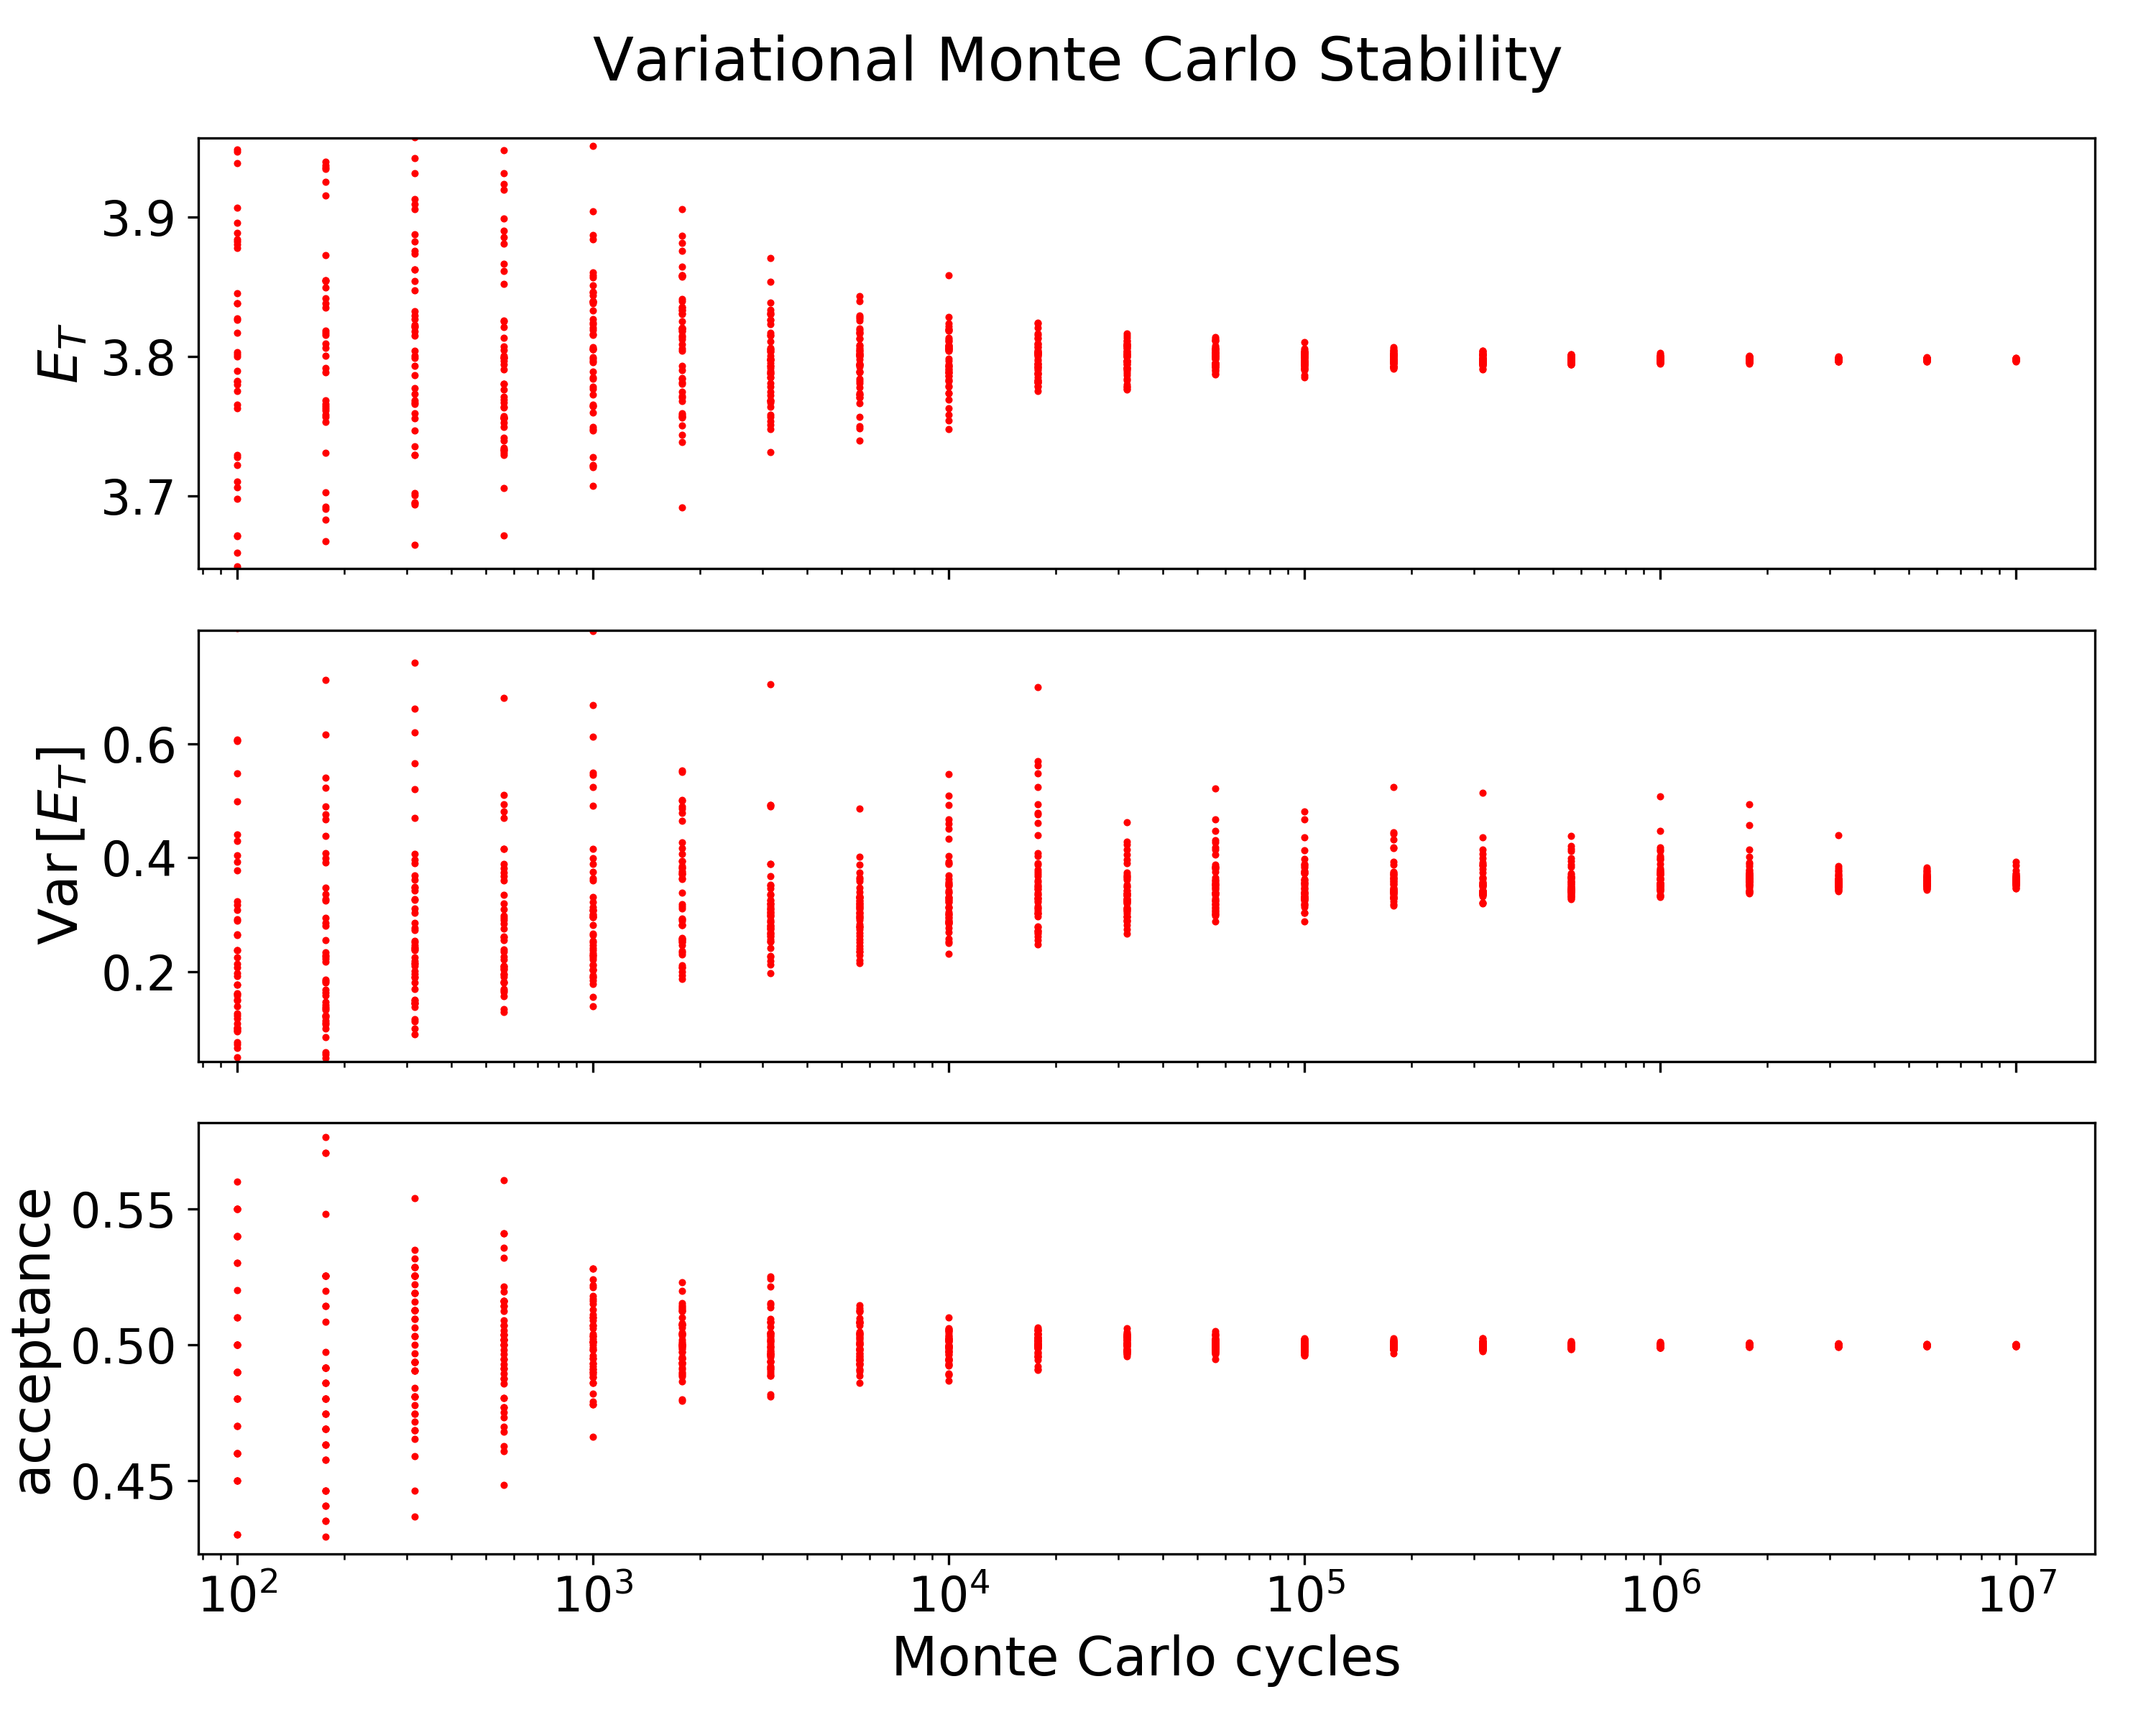
\includegraphics[scale=0.34]{../results/wave1/stability_2_edited.png}
\caption{The distribution of wave 1 trial energy and energy variance integrals as a function of the number of Monte Carlo cycles. The harmonic oscillator frequency is \(\omega=1\) and wave 1 variational parameter is \(\alpha=1\). The lower plot shows the average Monte Carlo acceptance ratio.}\label{fig:wave1_stability}
\end{figure}
\subsection{Experiment 2}
The results of the experiment are shown in figure \ref{fig:wave1_optimization}. Most notably, there is good agreement between the trial energy minimum and the energy variance minimum, in addition the acceptance ratio is fairly well-behaved in the region surrounding the energy minimum. The trial energy data was regressed against a polynomial of degree 5, as seen in figure \ref{fig:wave1_polyfit}, and found an energy minimum of about 3.773 Hartree using an optimal \(\alpha\) of about 0.8794. The expected electron separation using the optimal \(\alpha\) is shown in figure \ref{fig:wave1_separation}. As expected, the electrons are, on average, closer when the oscillator's strength is greater, and vice versa.

\begin{figure}
\centering
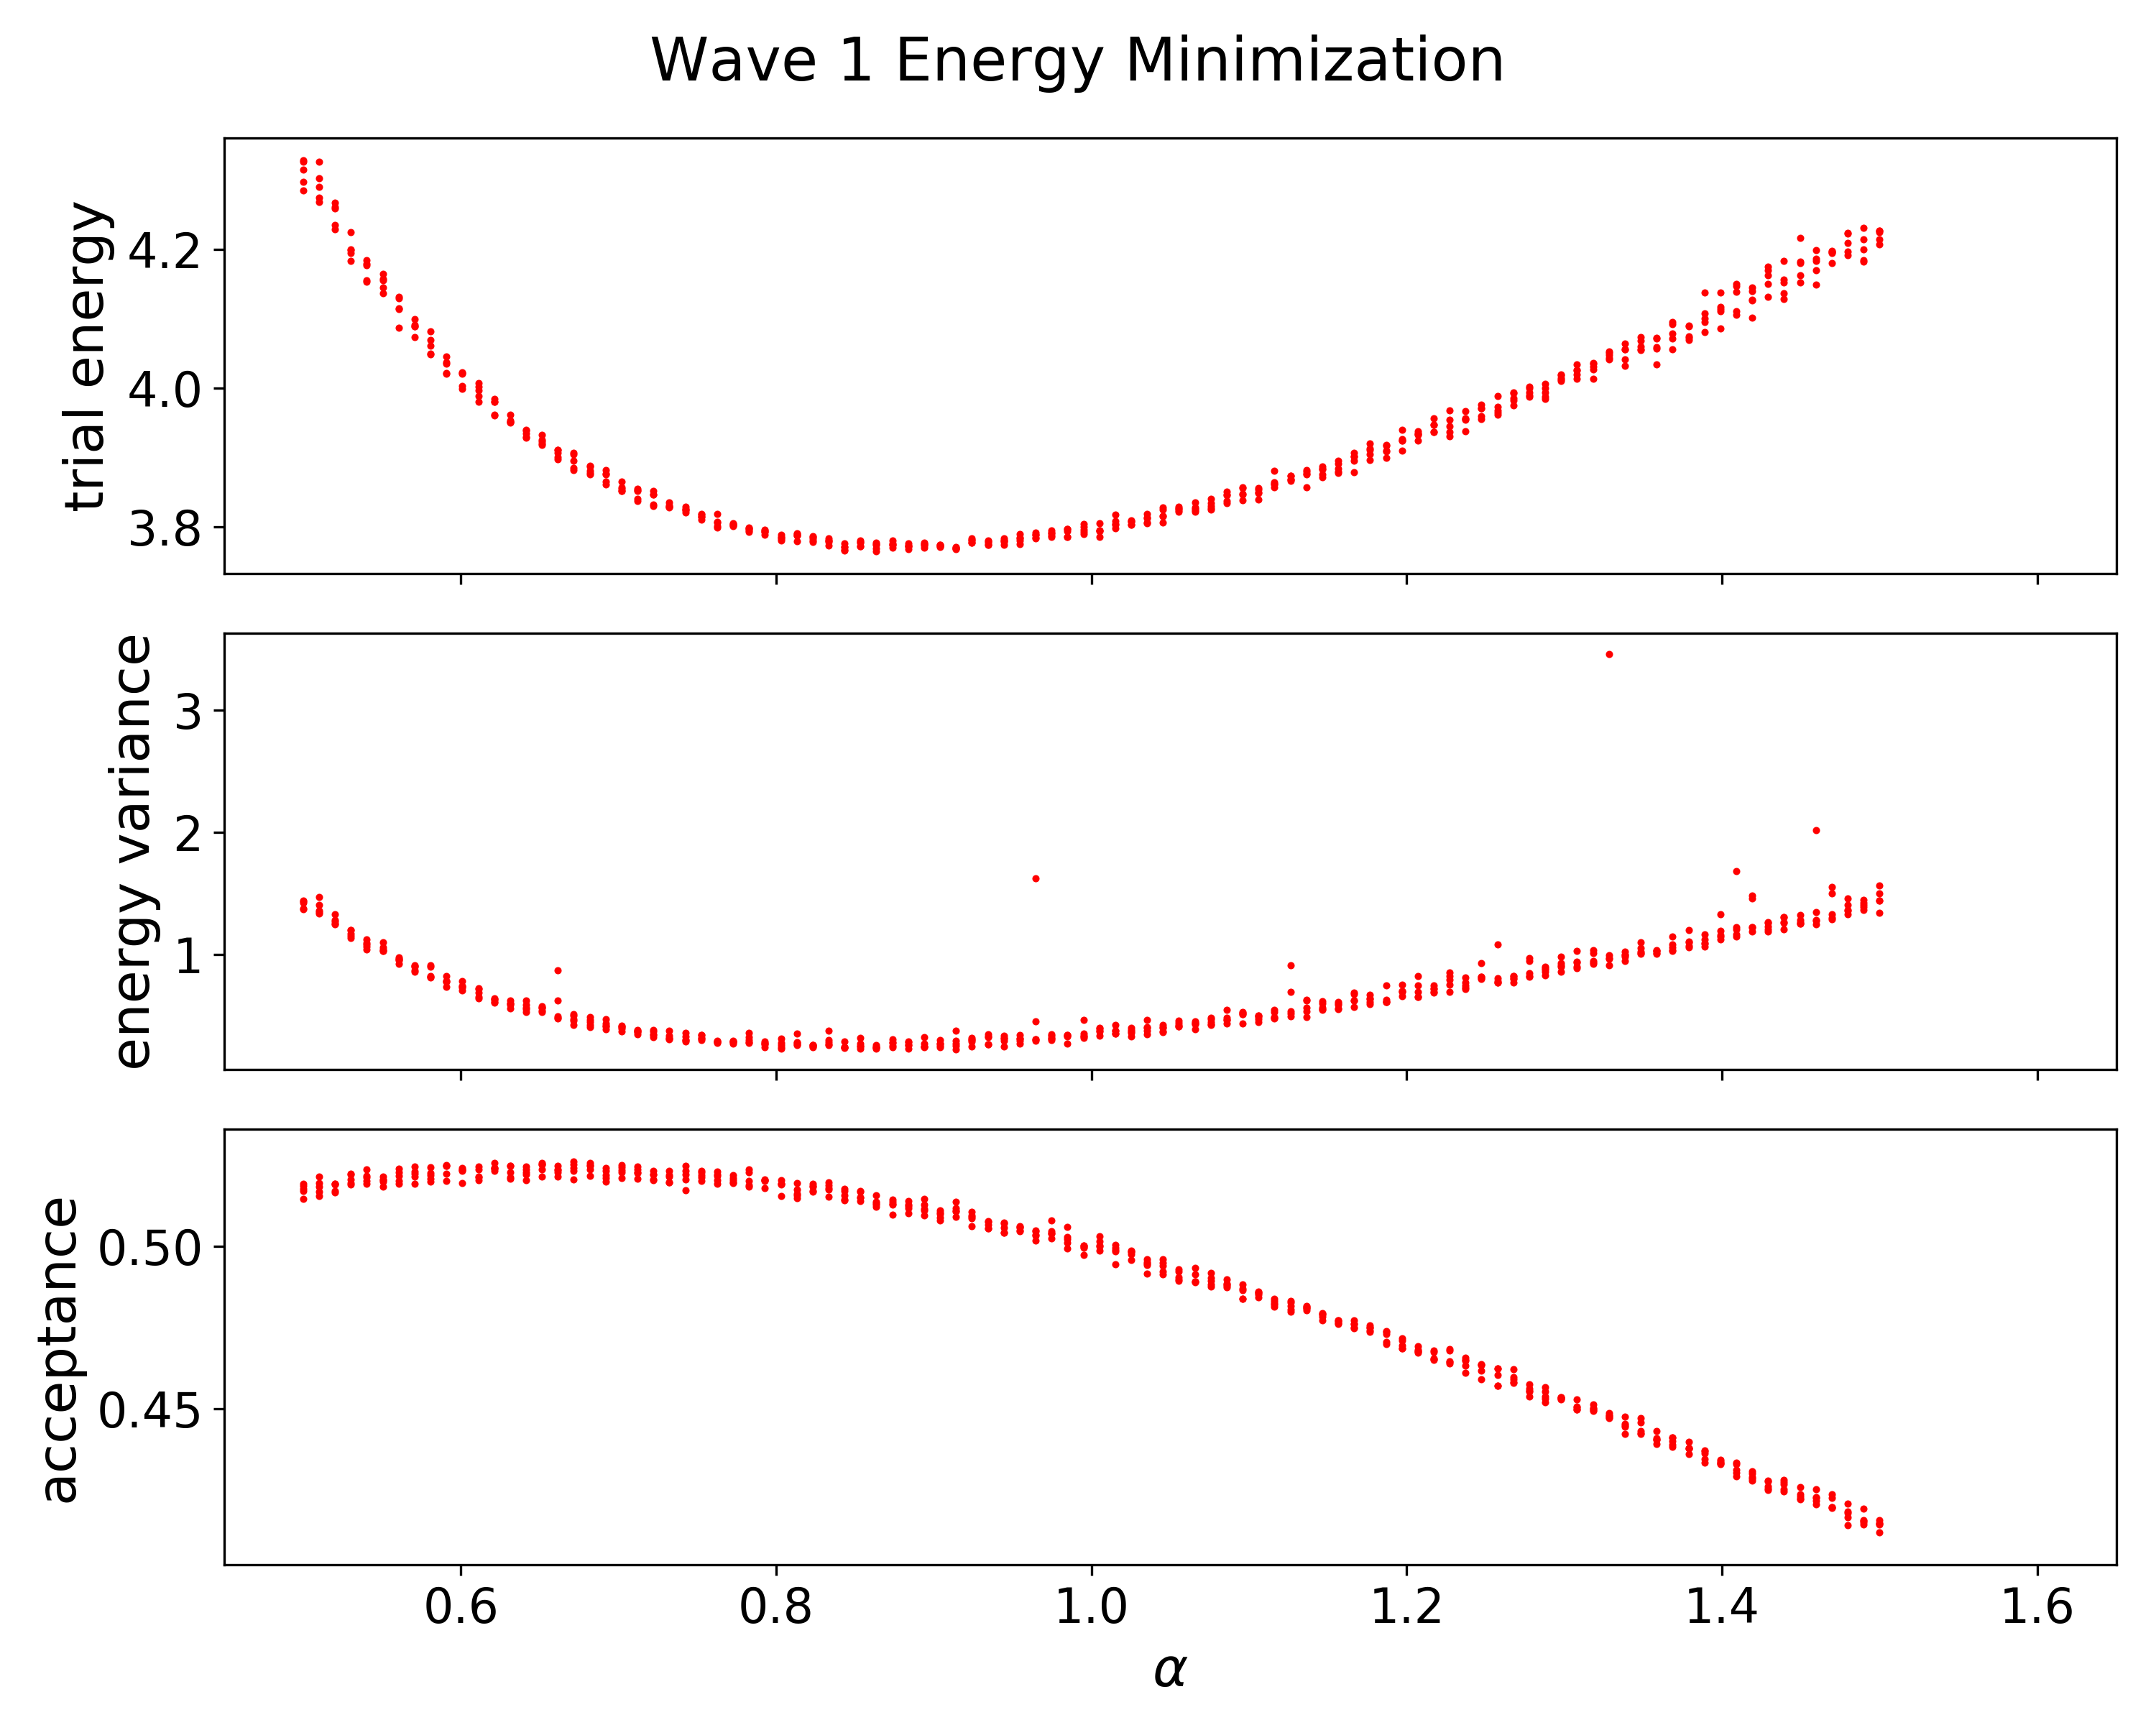
\includegraphics[scale=0.34]{../results/wave1/energy_minimization_2.png}
\caption{Variational Monte Carlo energy minimization of wave 1. The optimal \(\alpha\) is approximately 0.8794 with a corresponding energy minimum of about 3.773 Hartree.}\label{fig:wave1_optimization}
\end{figure}

\begin{figure}
\centering
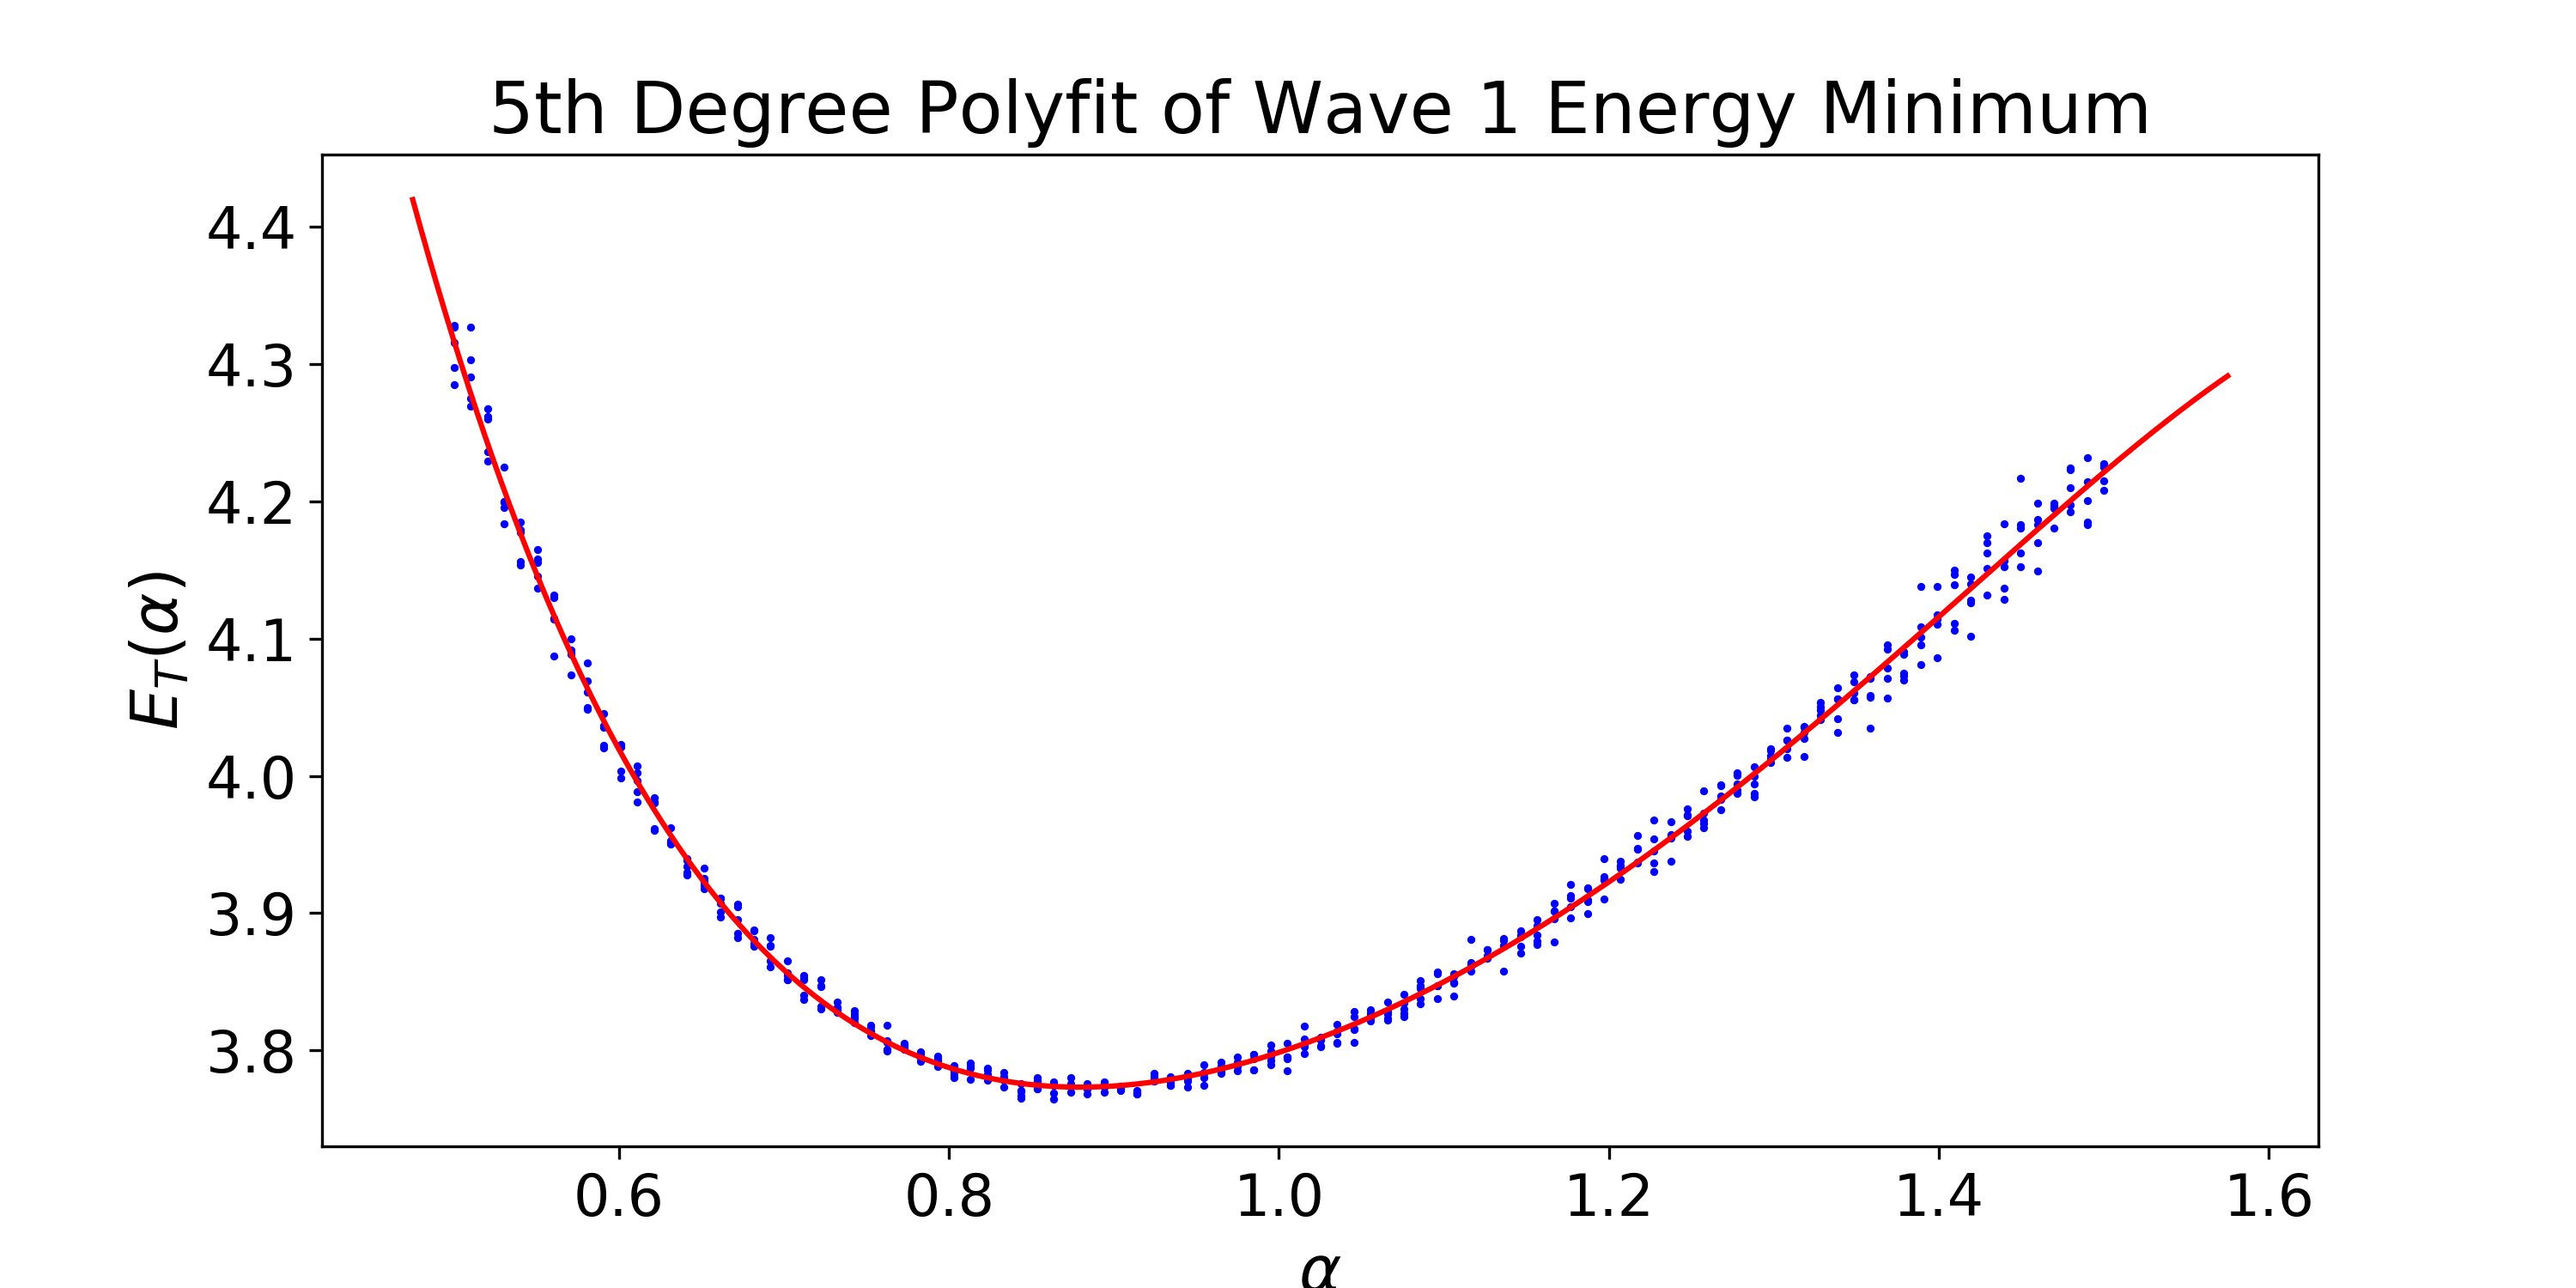
\includegraphics[scale=0.34]{../results/wave1/energy_minimum_deg5polyfit_2.png}
\caption{\(5^\text{th}\) degree polynomial interpolation of the trial energy data in figure \ref{fig:wave1_optimization}.}\label{fig:wave1_polyfit}
\end{figure}

\begin{figure}
\centering
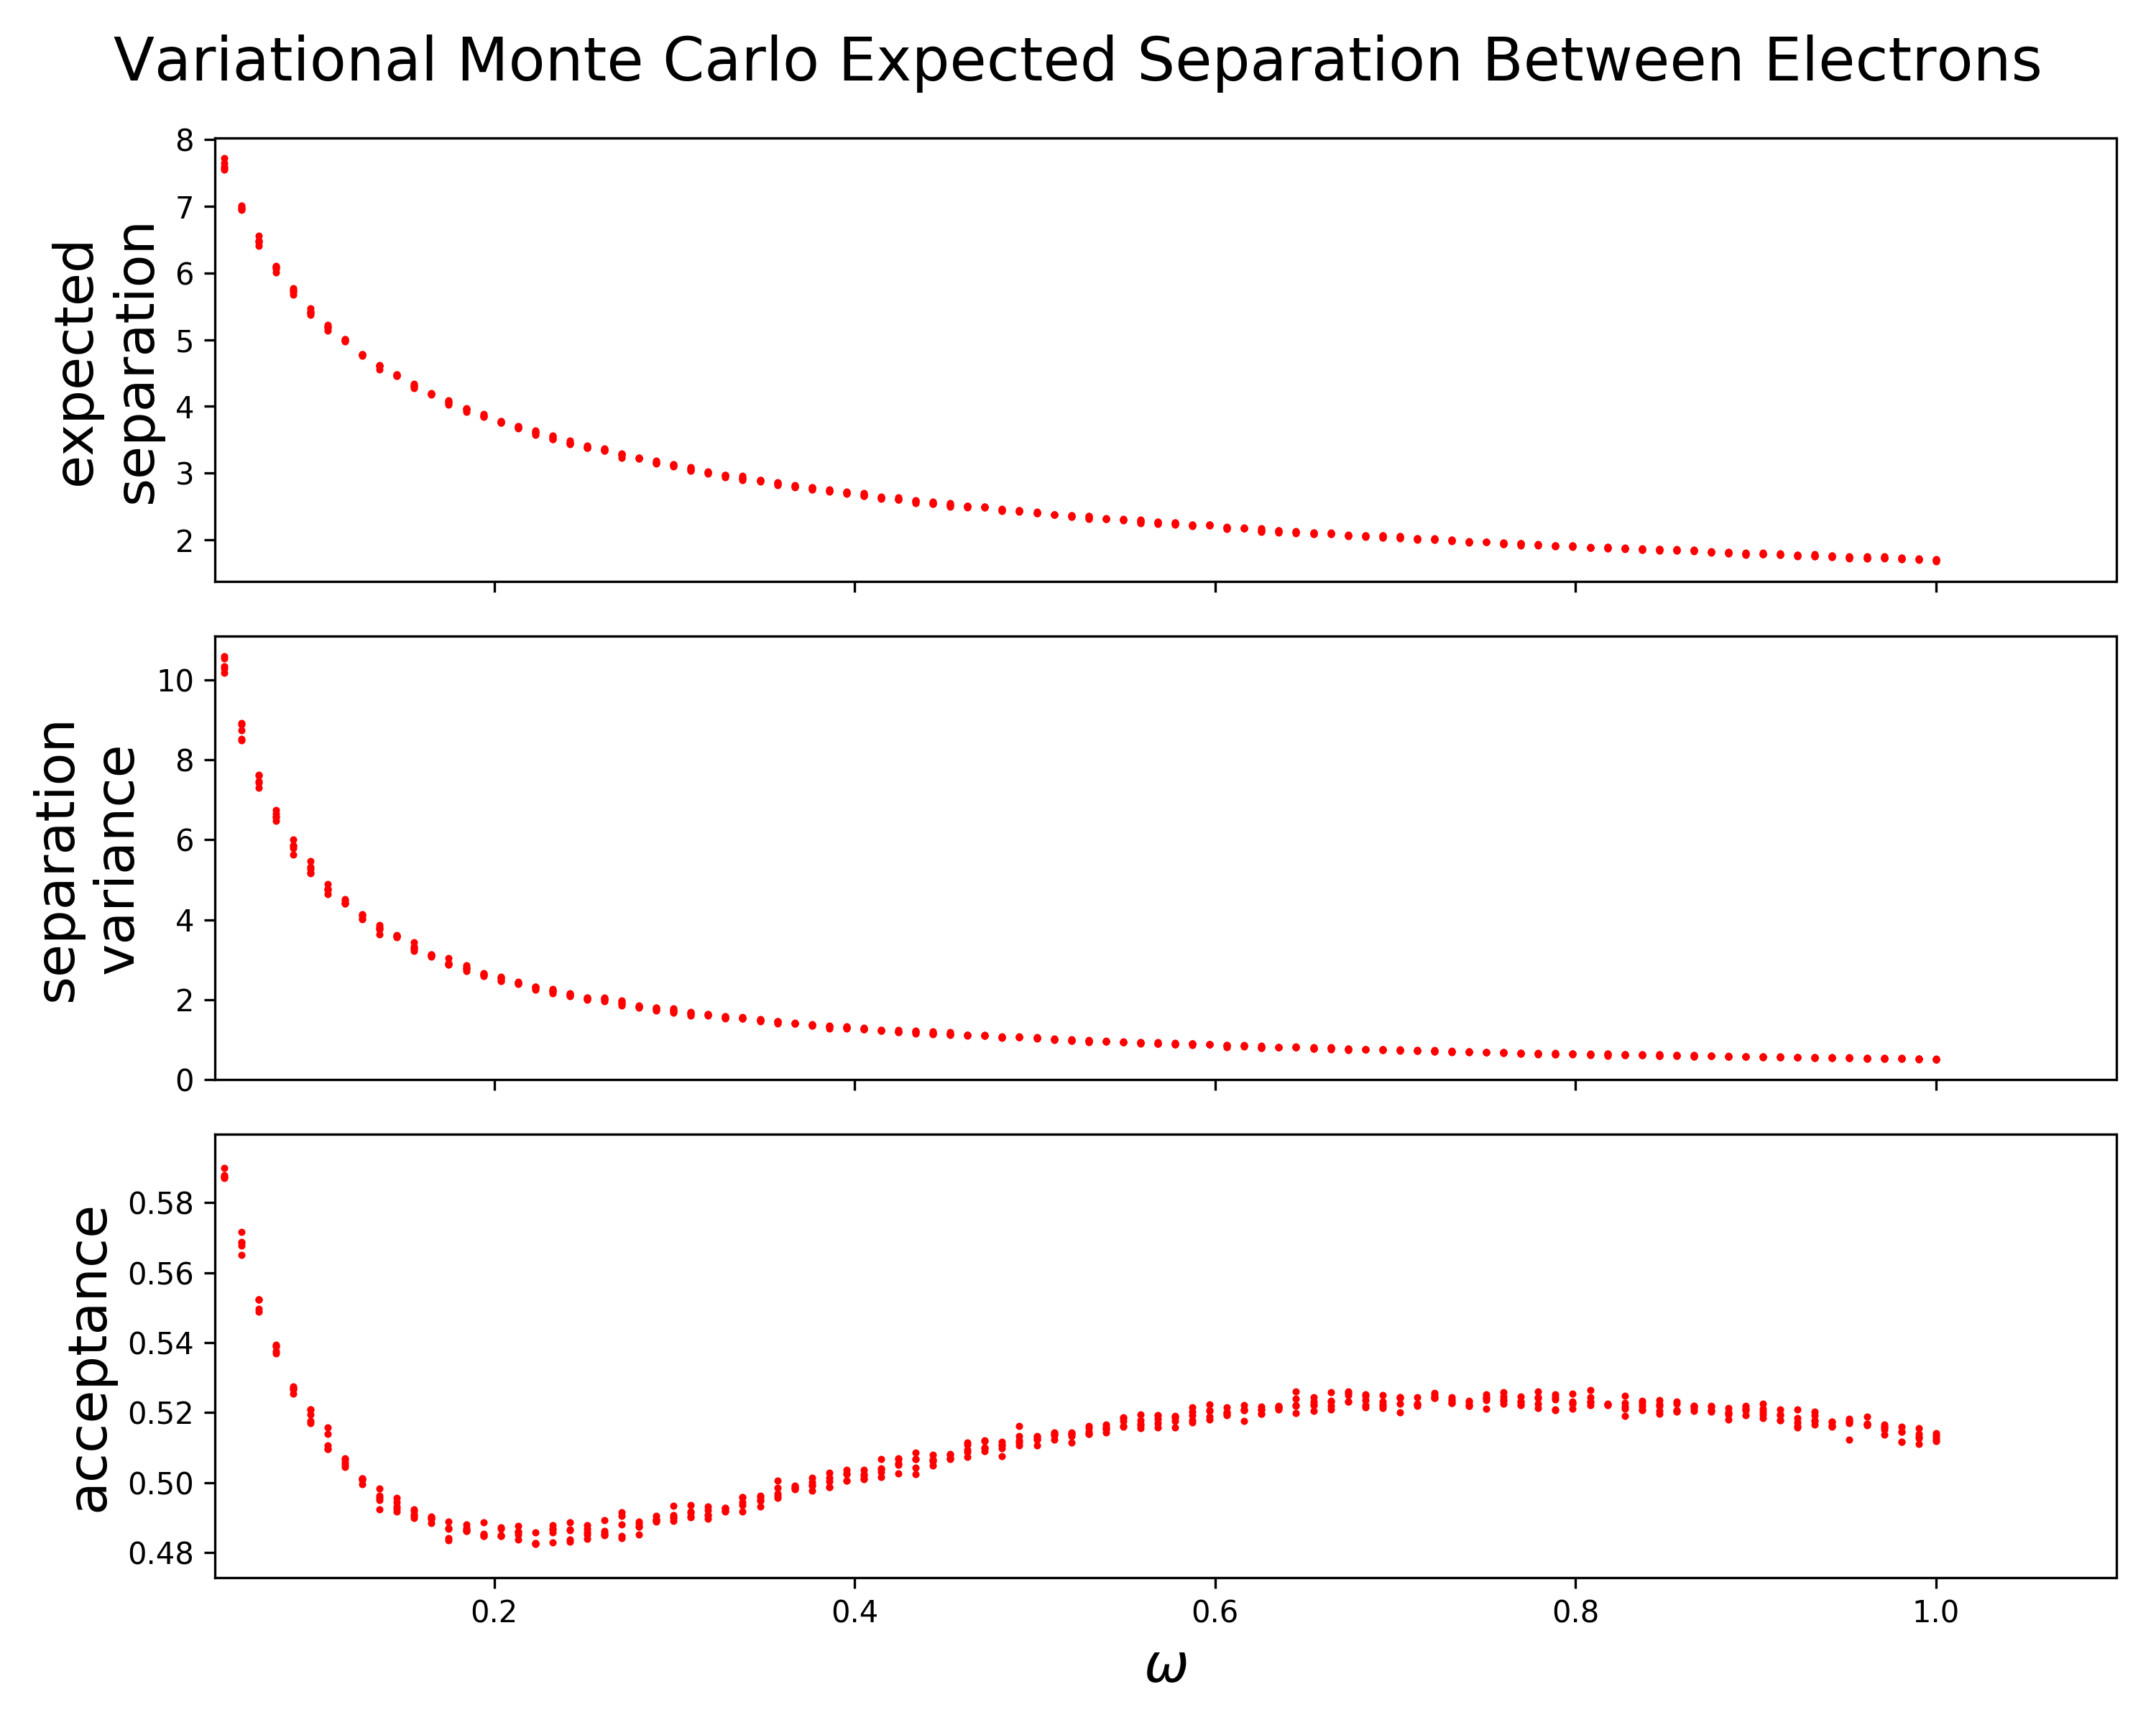
\includegraphics[scale=0.34]{../results/wave1/expected_separation_3.png}
\caption{The expected separation between the electrons using the optimal wave 1 variational parameter \(\alpha=0.8794\).}\label{fig:wave1_separation}
\end{figure}

\subsection{Experiment 3}
The results of the initial and final grid searches are shown in figure \ref{fig:wave2_optimization}, the intermediate grid searches can be found on the GitHub repository. The trial error was found to behave quite well with respect to a \(5^\text{th}\) order polynomial regressor, the polynomial interpolation is show in figure \ref{fig:wave2_polyfit}. The minimum energy of the polynomial interpolation was found to be about 3.730 Hartree, which is a lower than the wave 1 minimum energy by a 0.043 Hartre, using optimal variational parameters \(\alpha=0.9726\) and \(\beta=0.2405\). Using the optimal parameters the expected distance between the electrons was computed for the various oscillator frequencies, the results are shown in figure \ref{fig:wave2_separation}. The results are very similar to the results of experiment 2.


\onecolumngrid
\clearpage
~
\hspace*{8cm}
\begin{figure}[h!]
\centering
	\begin{subfigure}[b]{0.48\textwidth}
	\centering
	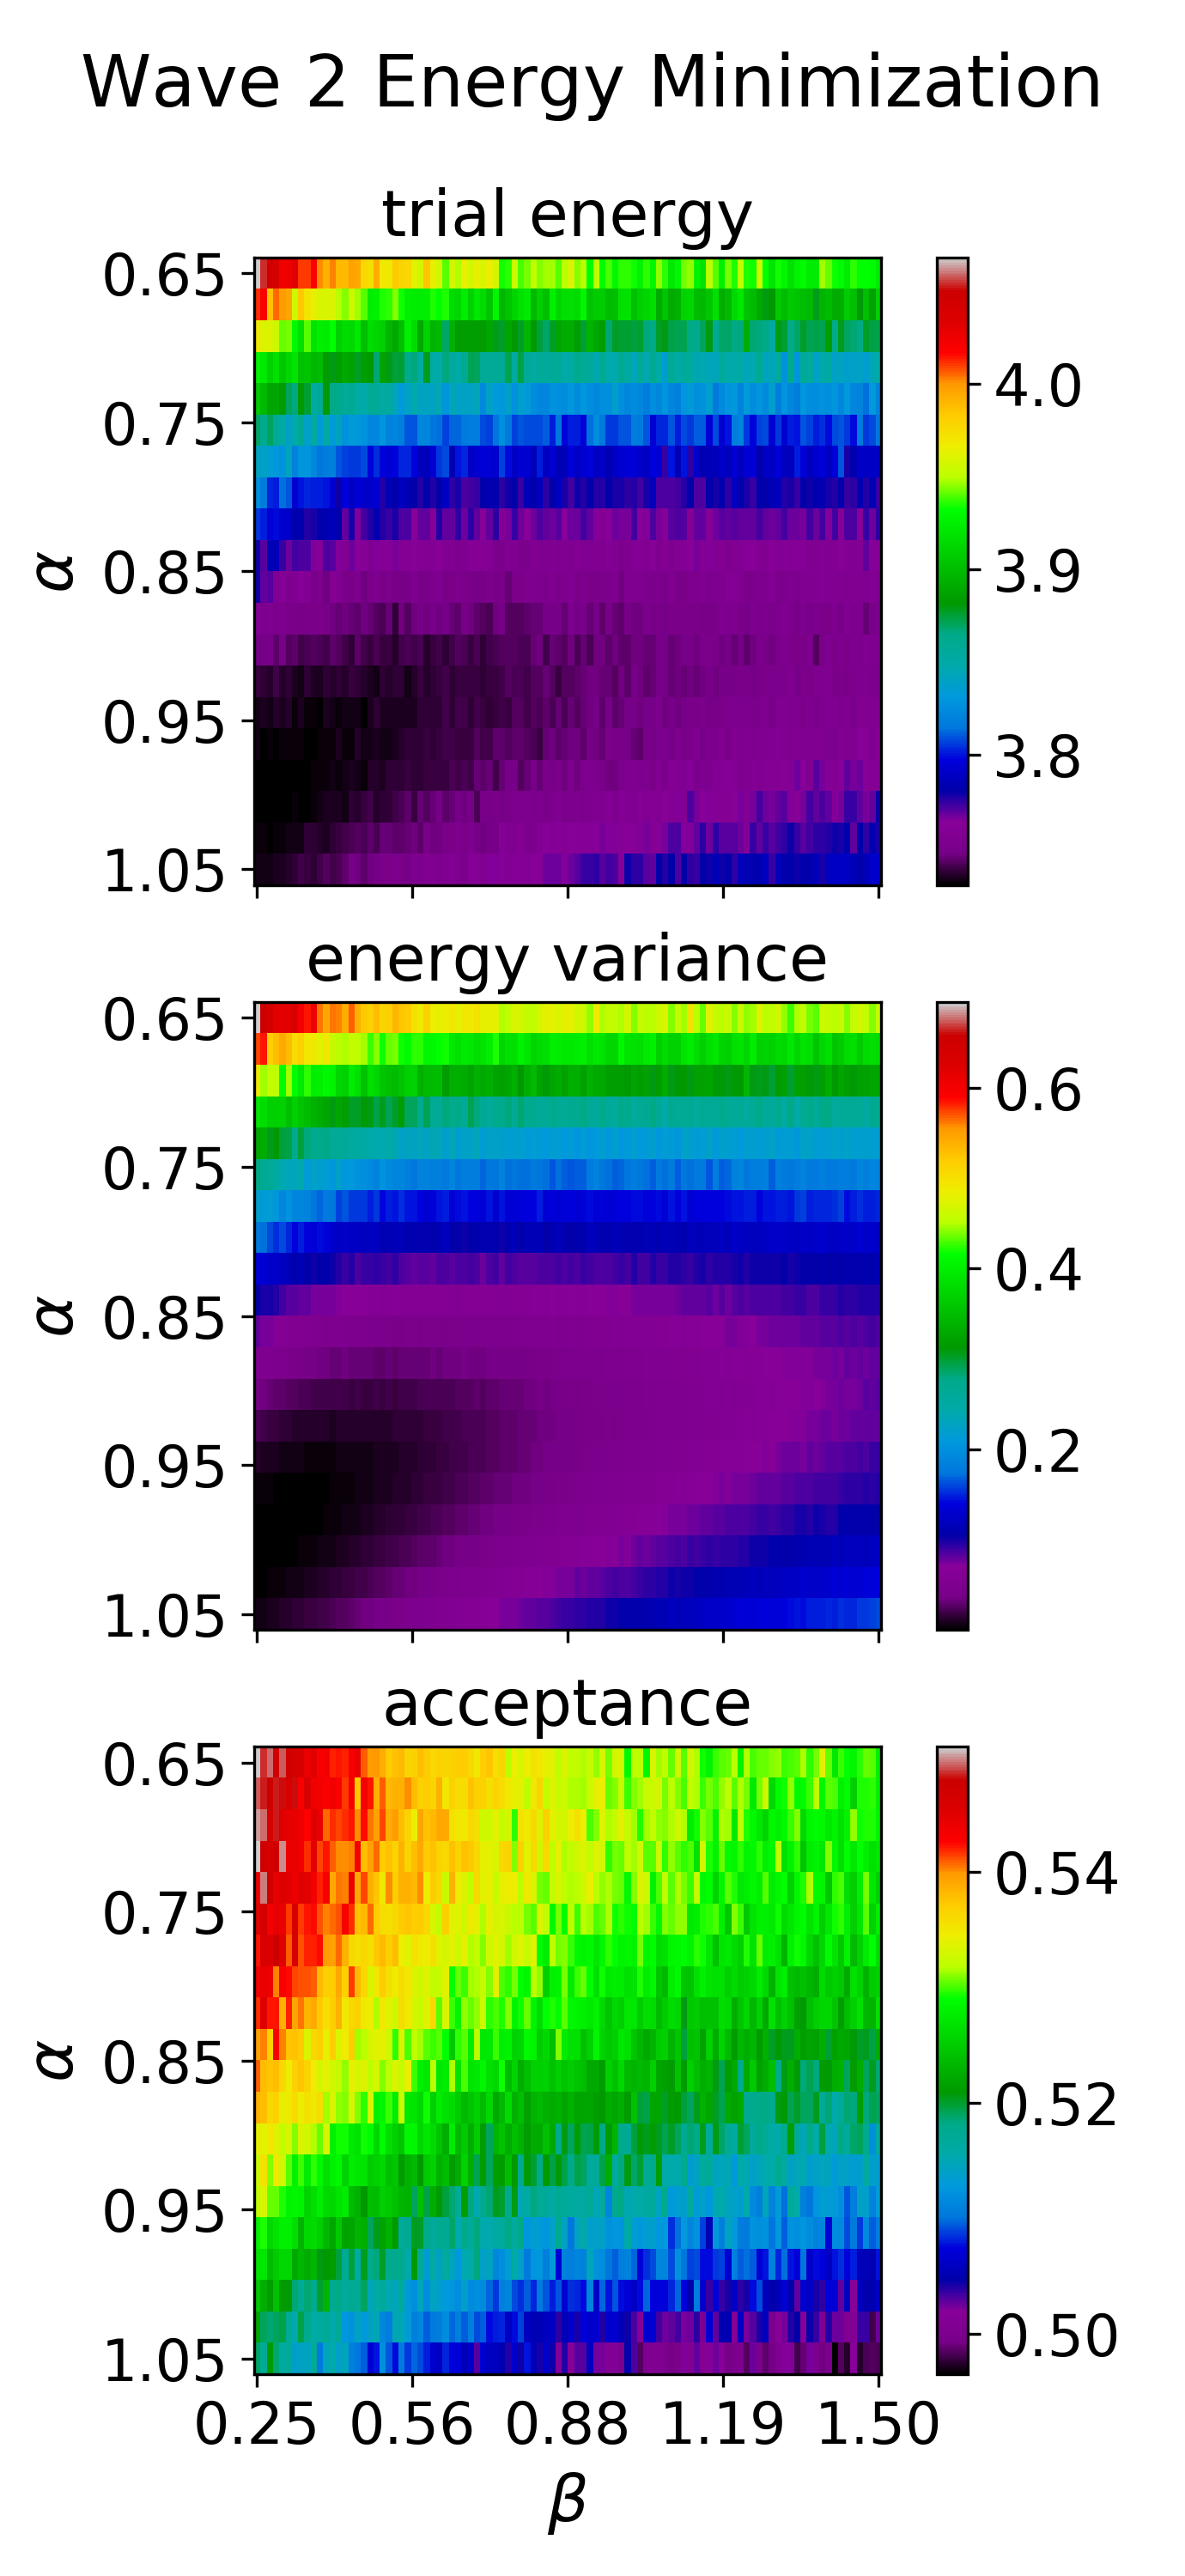
\includegraphics[scale=0.7]{../results/wave2/energy_minimization_1.png}
	\caption{\((\alpha,\beta)\in[0.65,1.05]\times[0.25,1.50]\)}\label{fig:wave2_optimization1}
	\end{subfigure}
	~
	\begin{subfigure}[b]{0.48\textwidth}
	\centering
	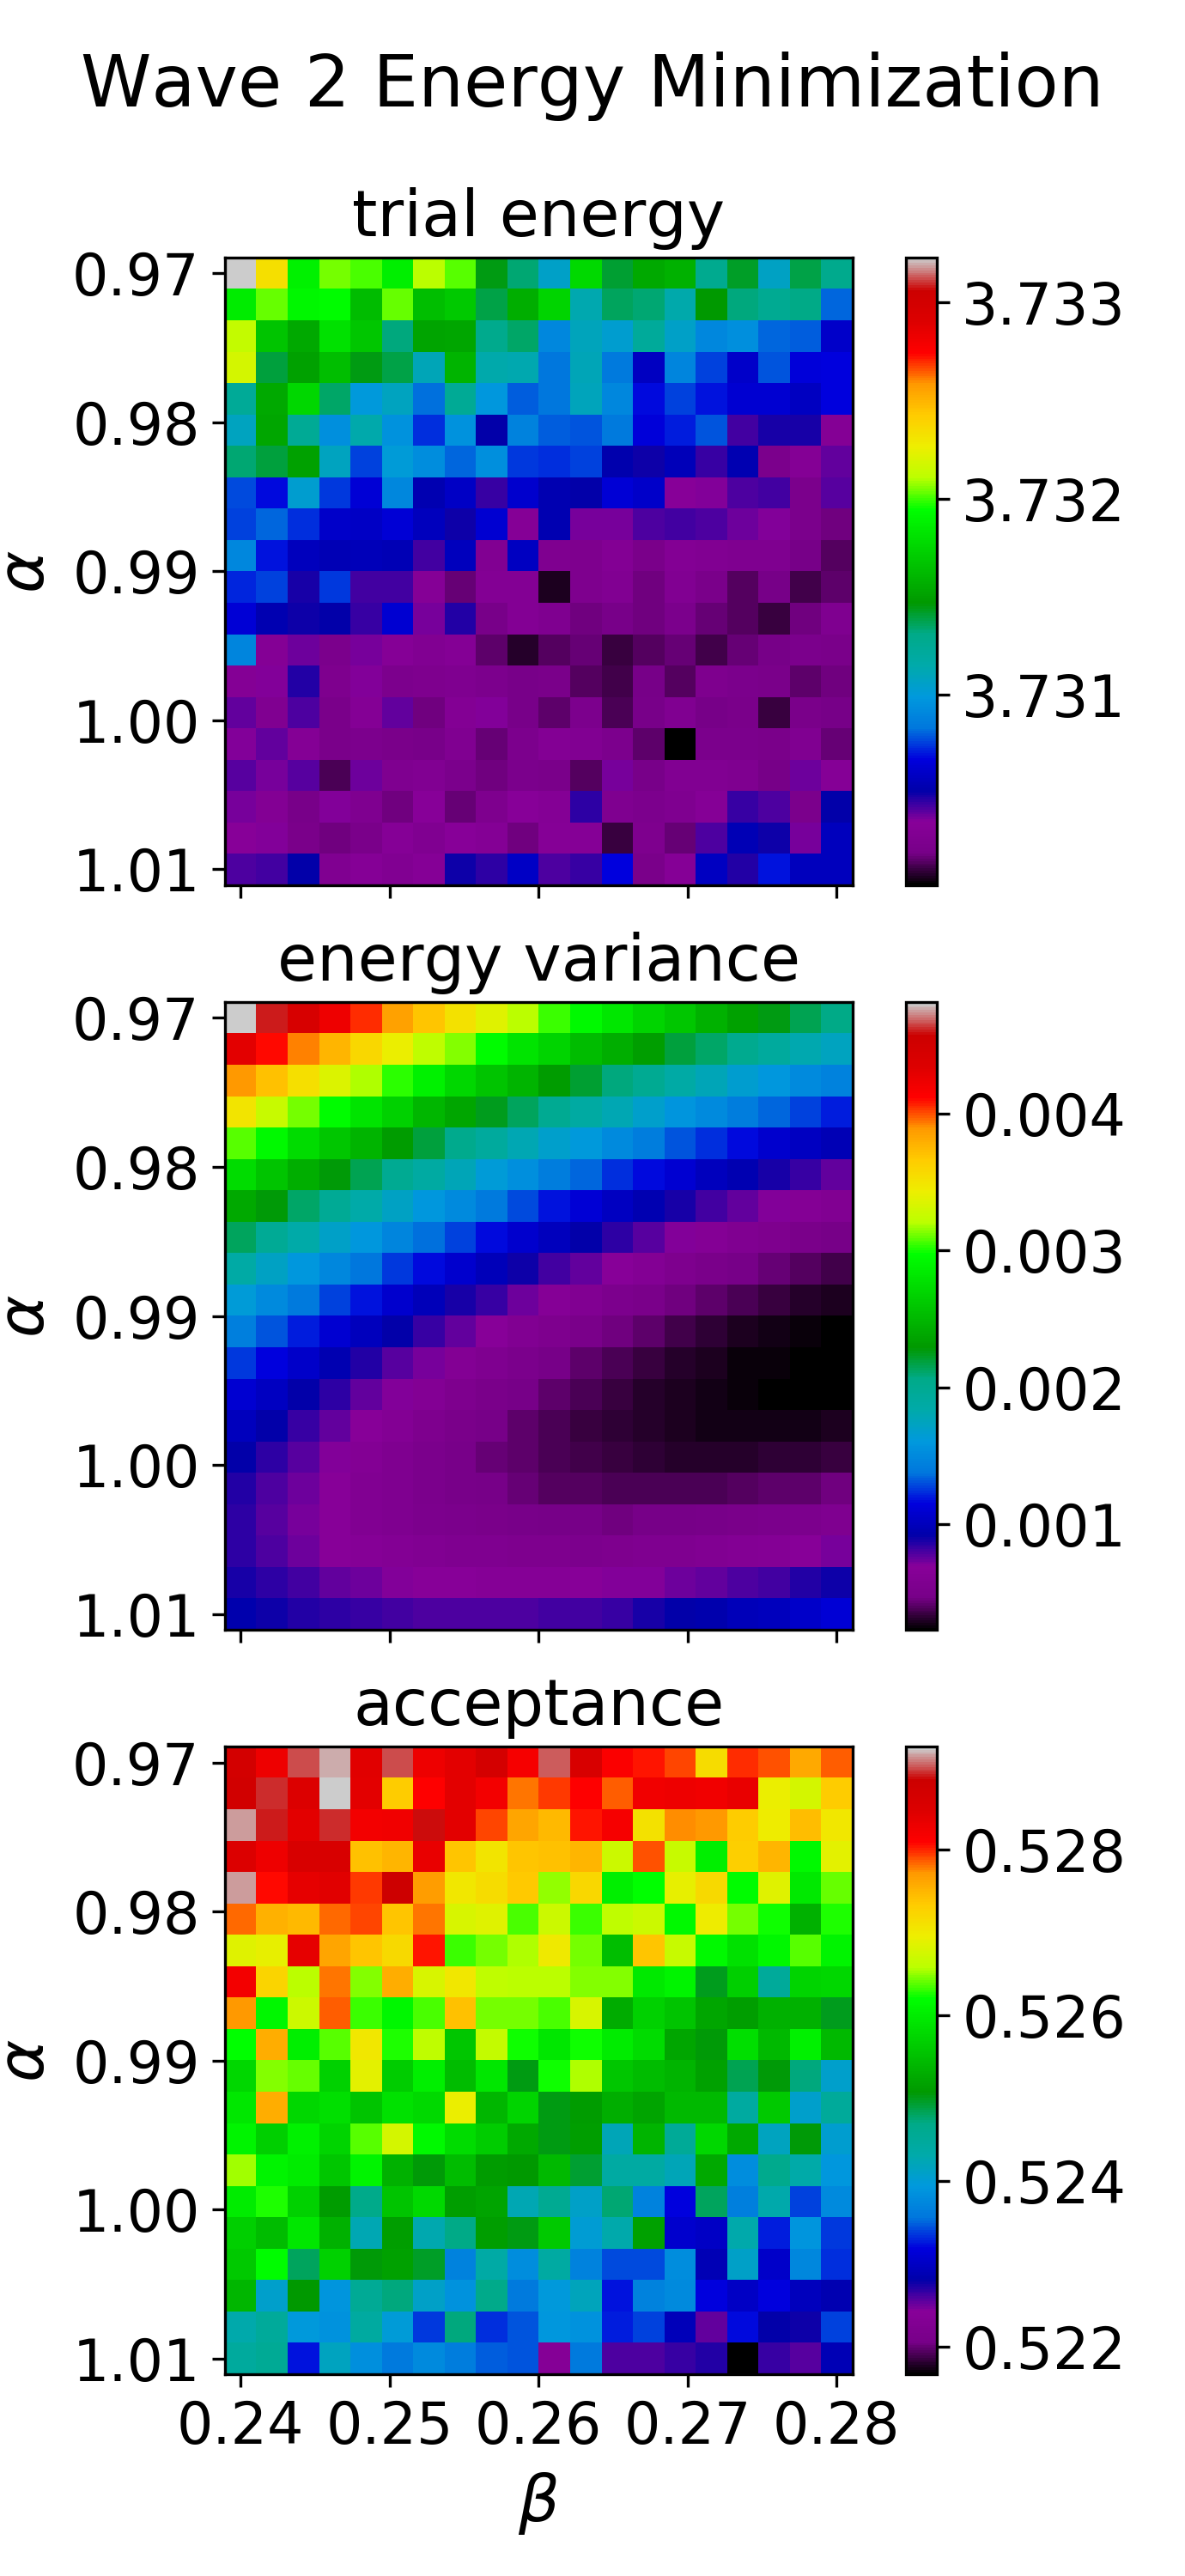
\includegraphics[scale=0.7]{../results/wave2/energy_minimization_5.png}
	\caption{\((\alpha,\beta)\in[0.972,1.012]\times[0.24,0.28]\)}\label{fig:wave2_optimization2}
	\end{subfigure}
\caption{Variational Monte Carlo energy minimization of wave 2. The two figures use different \((\alpha,\beta)\) grids.}\label{fig:wave2_optimization}
\end{figure}
\clearpage
\twocolumngrid

\begin{figure}
\centering
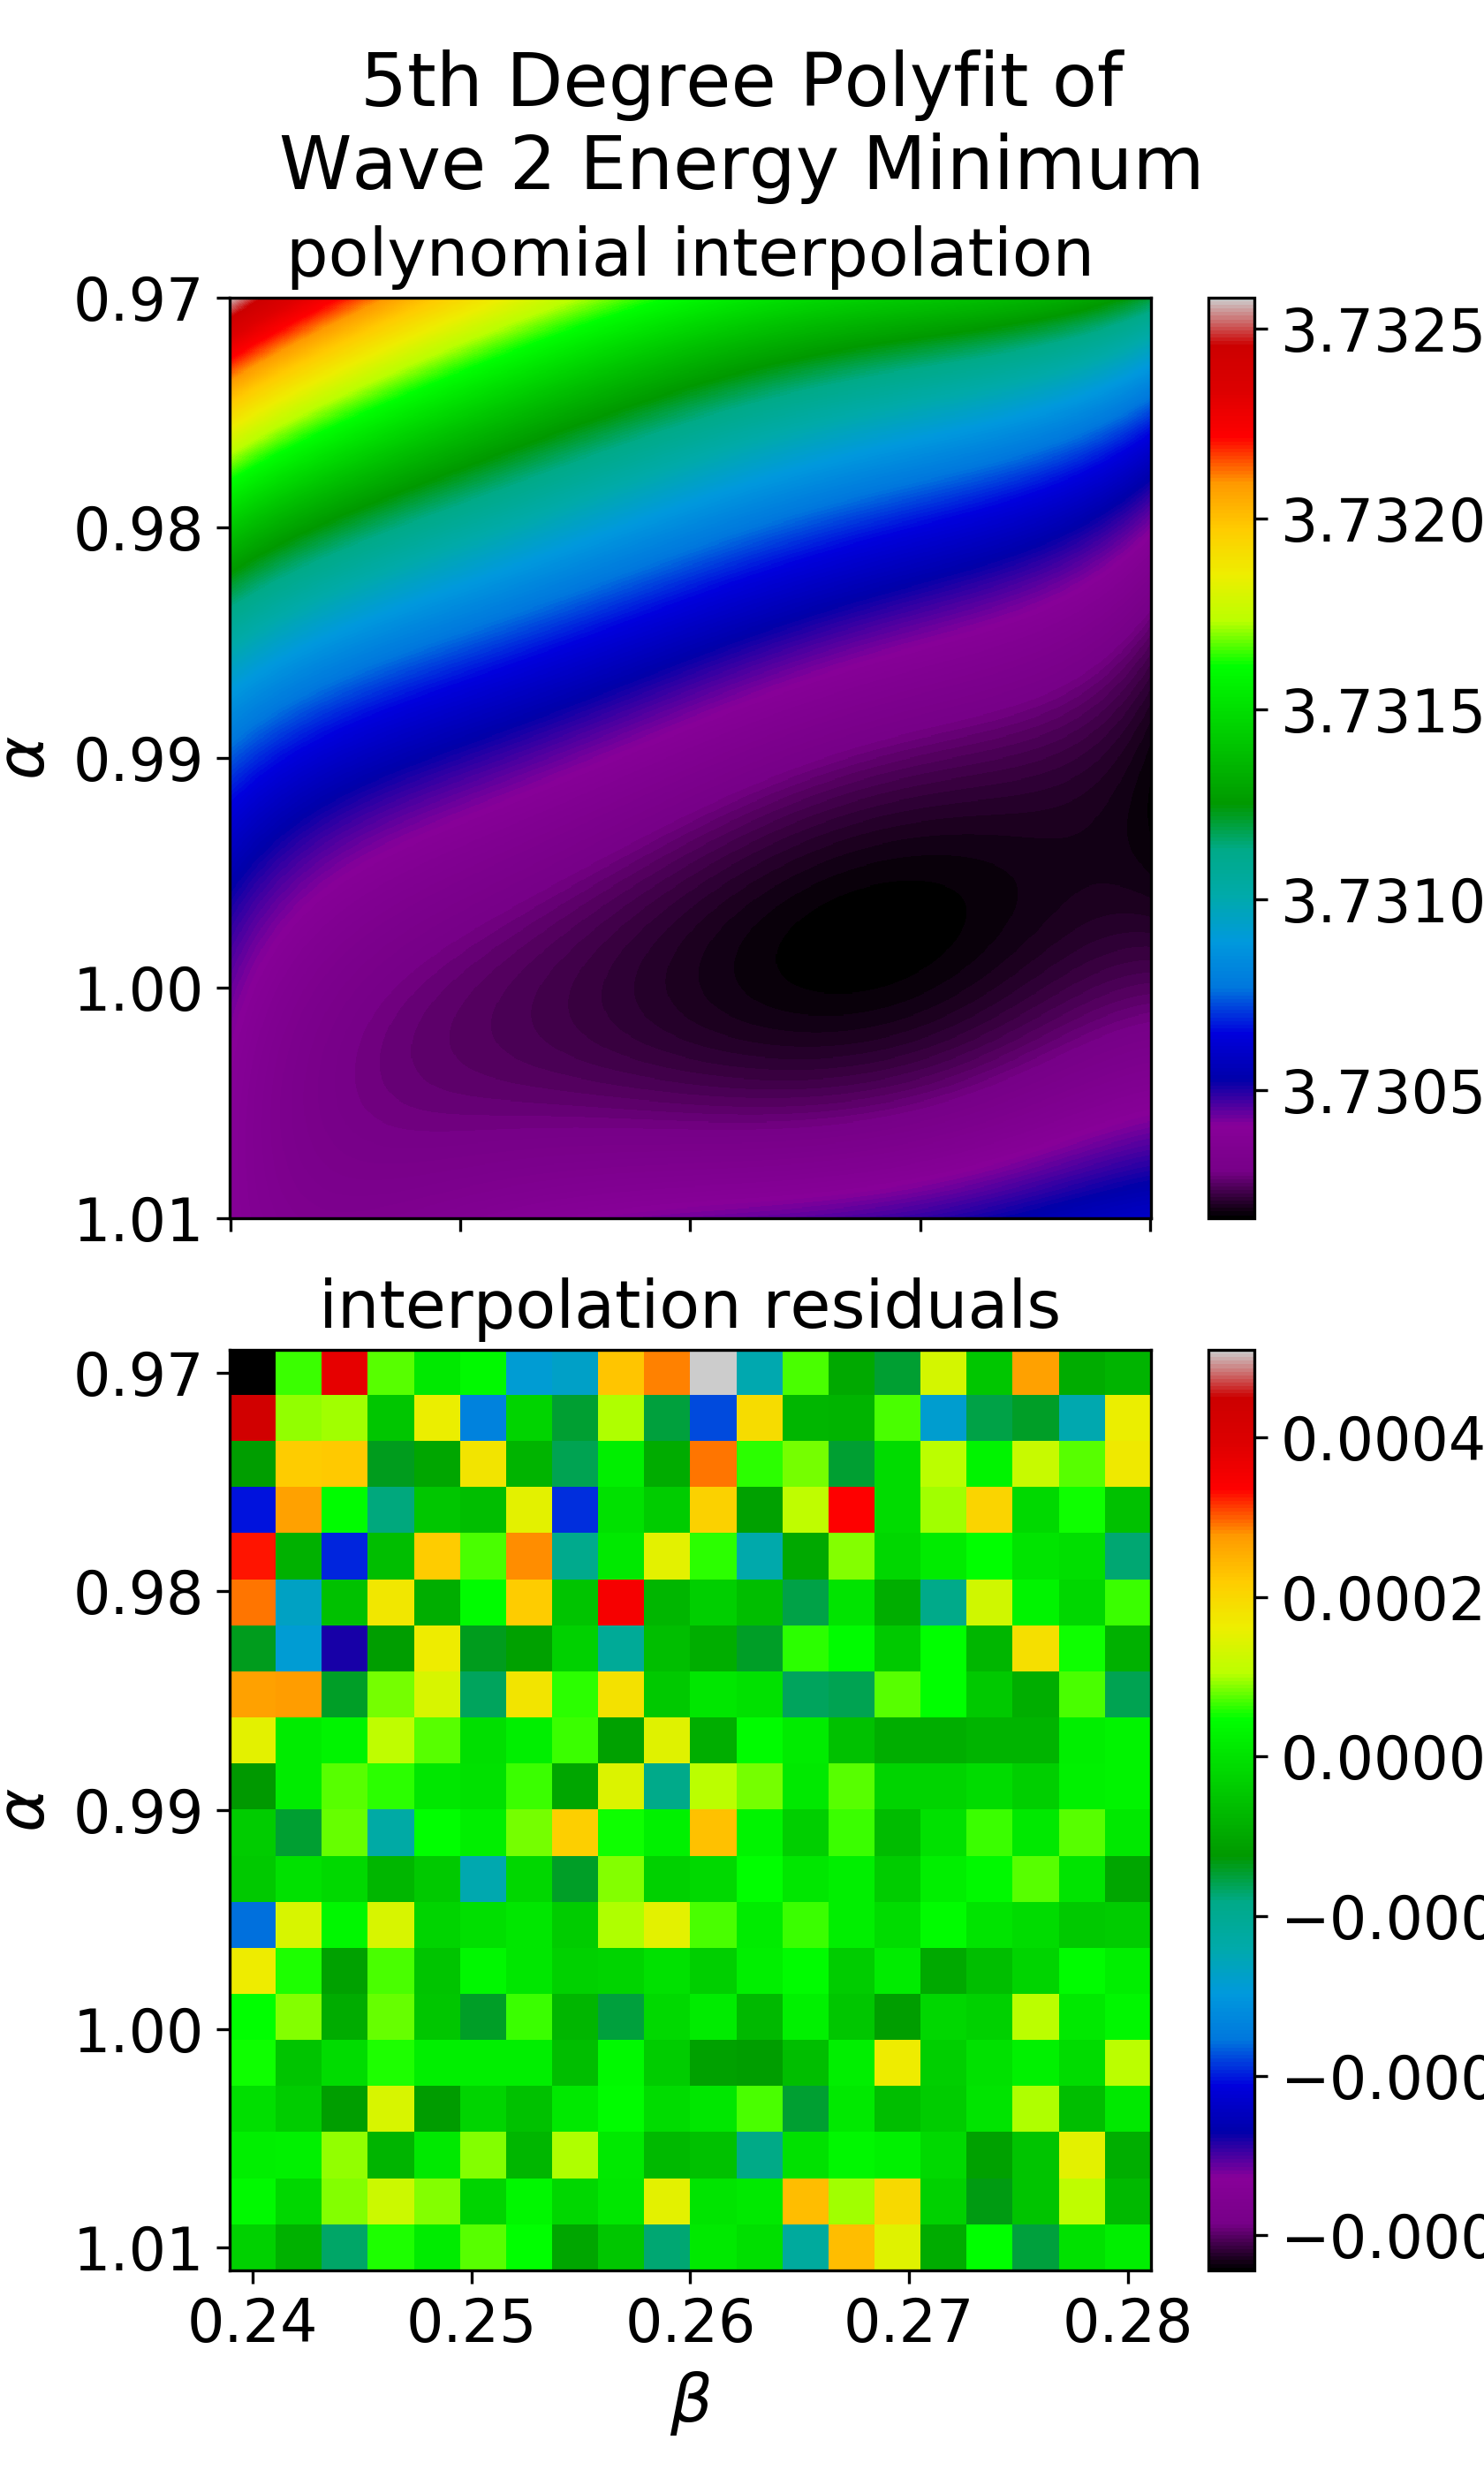
\includegraphics[scale=0.6]{../results/wave2/energy_minimization_deg5polyfit_5.png}
\caption{\(5^\text{th}\) degree polynomial interpolation of the trial energy data in figure \ref{fig:wave2_optimization2}. Note that the colours of the polynomial interpolation does not correspond to the colours in \ref{fig:wave2_optimization2}, despite use of the same matplotlib colormap.}\label{fig:wave2_polyfit}
\end{figure}

\begin{figure}
\centering
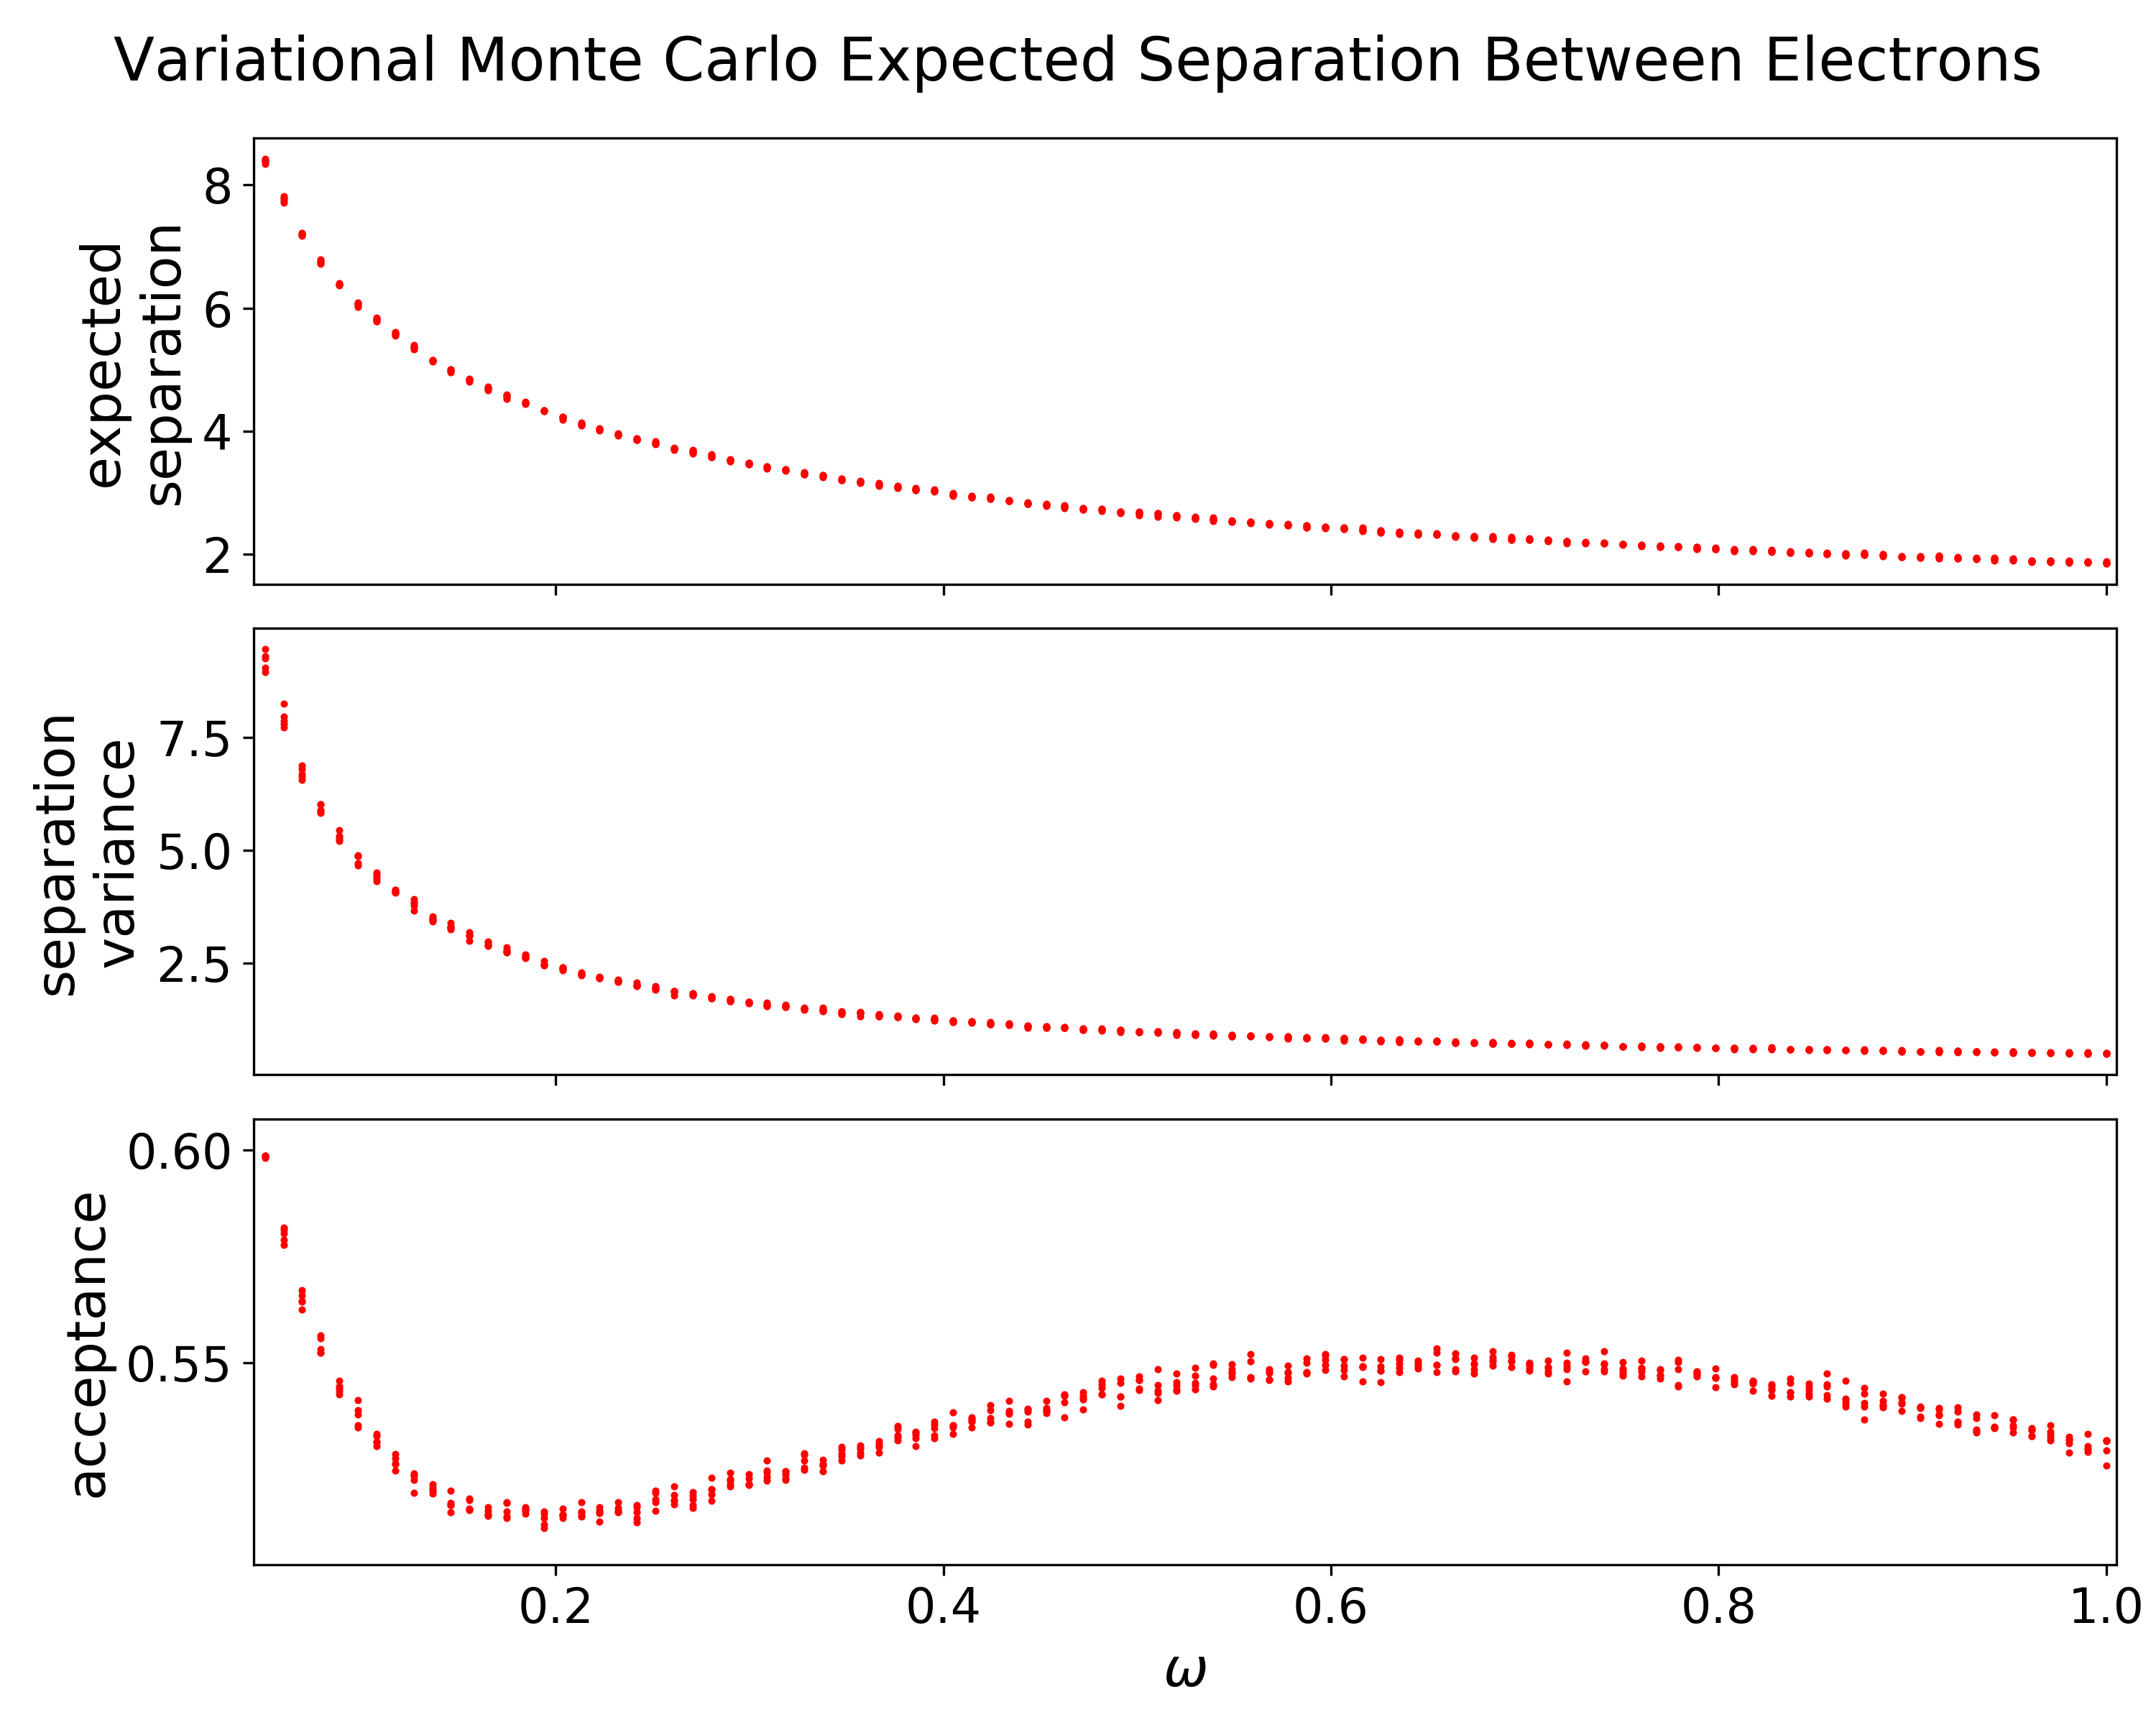
\includegraphics[scale=0.34]{../results/wave2/expected_separation_1_edited.png}
\caption{The expected separation between the electrons using the optimal wave 2 variational parameters \(\alpha=0.9726\) and \(\beta=0.2405\).}\label{fig:wave2_separation}
\end{figure}

\subsection{Experiment 4}
The electron-electron energy balance is shown in figure \ref{fig:virial}. The non-interacting data is very stable for all \(\omega\), which is reasonble given the fact that is constant for the ground state. The interacting data sets both increase with decreasing \(\omega\), especially the interacting wave 1 dat set grows faster than the wave 2 data set.

\begin{figure}
\centering
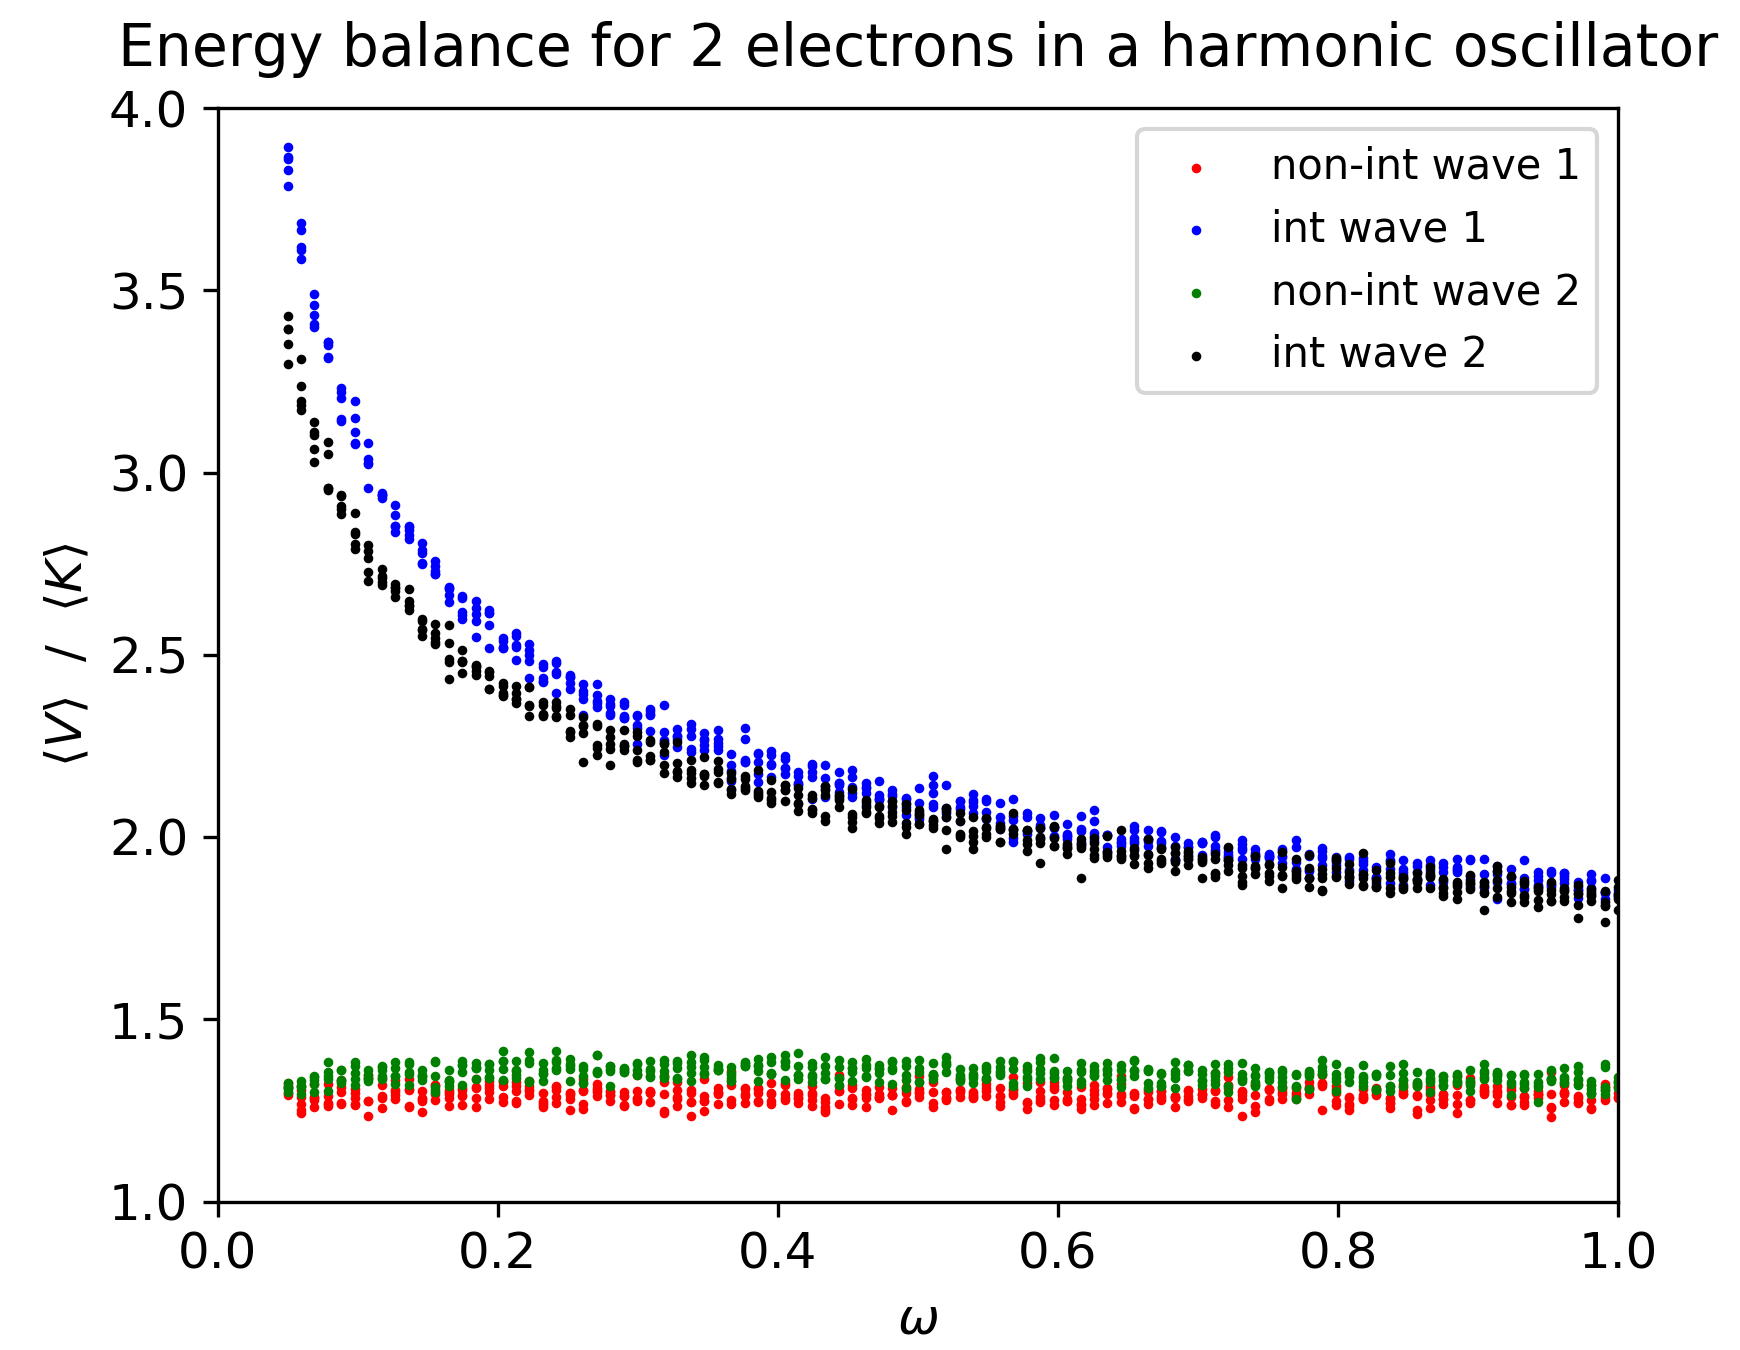
\includegraphics[scale=0.5]{../results/virial/energy_balance_2.png}
\caption{The balance between the potential and kinetic energy of two electrons in a harmonic oscillator. The four data sets refer to wave 1 and 2, with or without a Coulomb interaction.}\label{fig:virial}
\end{figure}



\section{Discussion}

\section{Conclusion}

%\bibliographystyle{plain}
%\bibliography{references.bib}


~
\clearpage
\appendix

\onecolumngrid
\section{Miscellaneous Material}\label{app:misc_material}

\end{document}